\subsection{Overview}
CLup's architecture is layered as follows:
\begin{itemize}
	\item \textbf{Presentation layer} (P) handles the interaction with users. It contains the interfaces able to communicate with them and it is responsible for rendering of the information. Its scope is to make understandable the functions of the application to the customers.
	\item \textbf{Application layer} (A) takes care of the functions to be provided for the users. It also coordinates the work of the application, making logical decisions and moving data between	the other two layers.
	\item \textbf{Data access layer }(D) which takes care of the information management, database access control. It also handles data retrieval and passes them to upper level layers.
\end{itemize}
 
The architecture style chosen for CLup is the \textbf{multi-tier} one.
As previously anticipated in the Requirements Analysis and Specifications Document, there will be at least one server for each one of the following interest areas:
\begin{itemize}
    \item Bookings
    \item Queues
    \item Notifications
    \item Stores
    \item Staff members
    \item Customers
\end{itemize}

This is mainly done to distribute workload as well as making the overall system more robust.

There will be also at least two servers for the two following functionalities:
\begin{itemize}
    \item Customer related functionalities
    \item Staff related functionalities
\end{itemize}
The bookings, queue and notifications databases will be distributed and replicated all over the entire store list. Each store will have its own instance of bookings, queue and notifications database while a central logic server will act as a request redirector towards them whenever needed.\\

In Figure \ref{fig:HLArch} is represented the high-level architecture of the system: customers clients, through an internet connection, can connect to Clup's App Servers, which represent the A layer of the Clup customer side. Client's operations store o retrieve information from People DB Servers or directly from the Local DB of the store, depending by the kind of information. Staff clients instead are connected through a LAN connection to their Local Web Server, who will redirect their requests to the Staff Operations Manager server. This machine is expected to process the logic of requests and then submit them to the Local Application server who also store or retrieve the information from the Local DB or People DB server depending by the situation. Local Application Server is fundamental also for Totem users, in fact the Totem rely on this server for its requests. Staff clients may need to connect to Clup Centralized Hardware, to do this they need an internet connection to get in contact with the dedicated Central Web server, the P layer who then send the request to the Store Operations Manager, the A layer. This server stores and retrieves information from Stores DB servers
\begin{figure}[h!]
	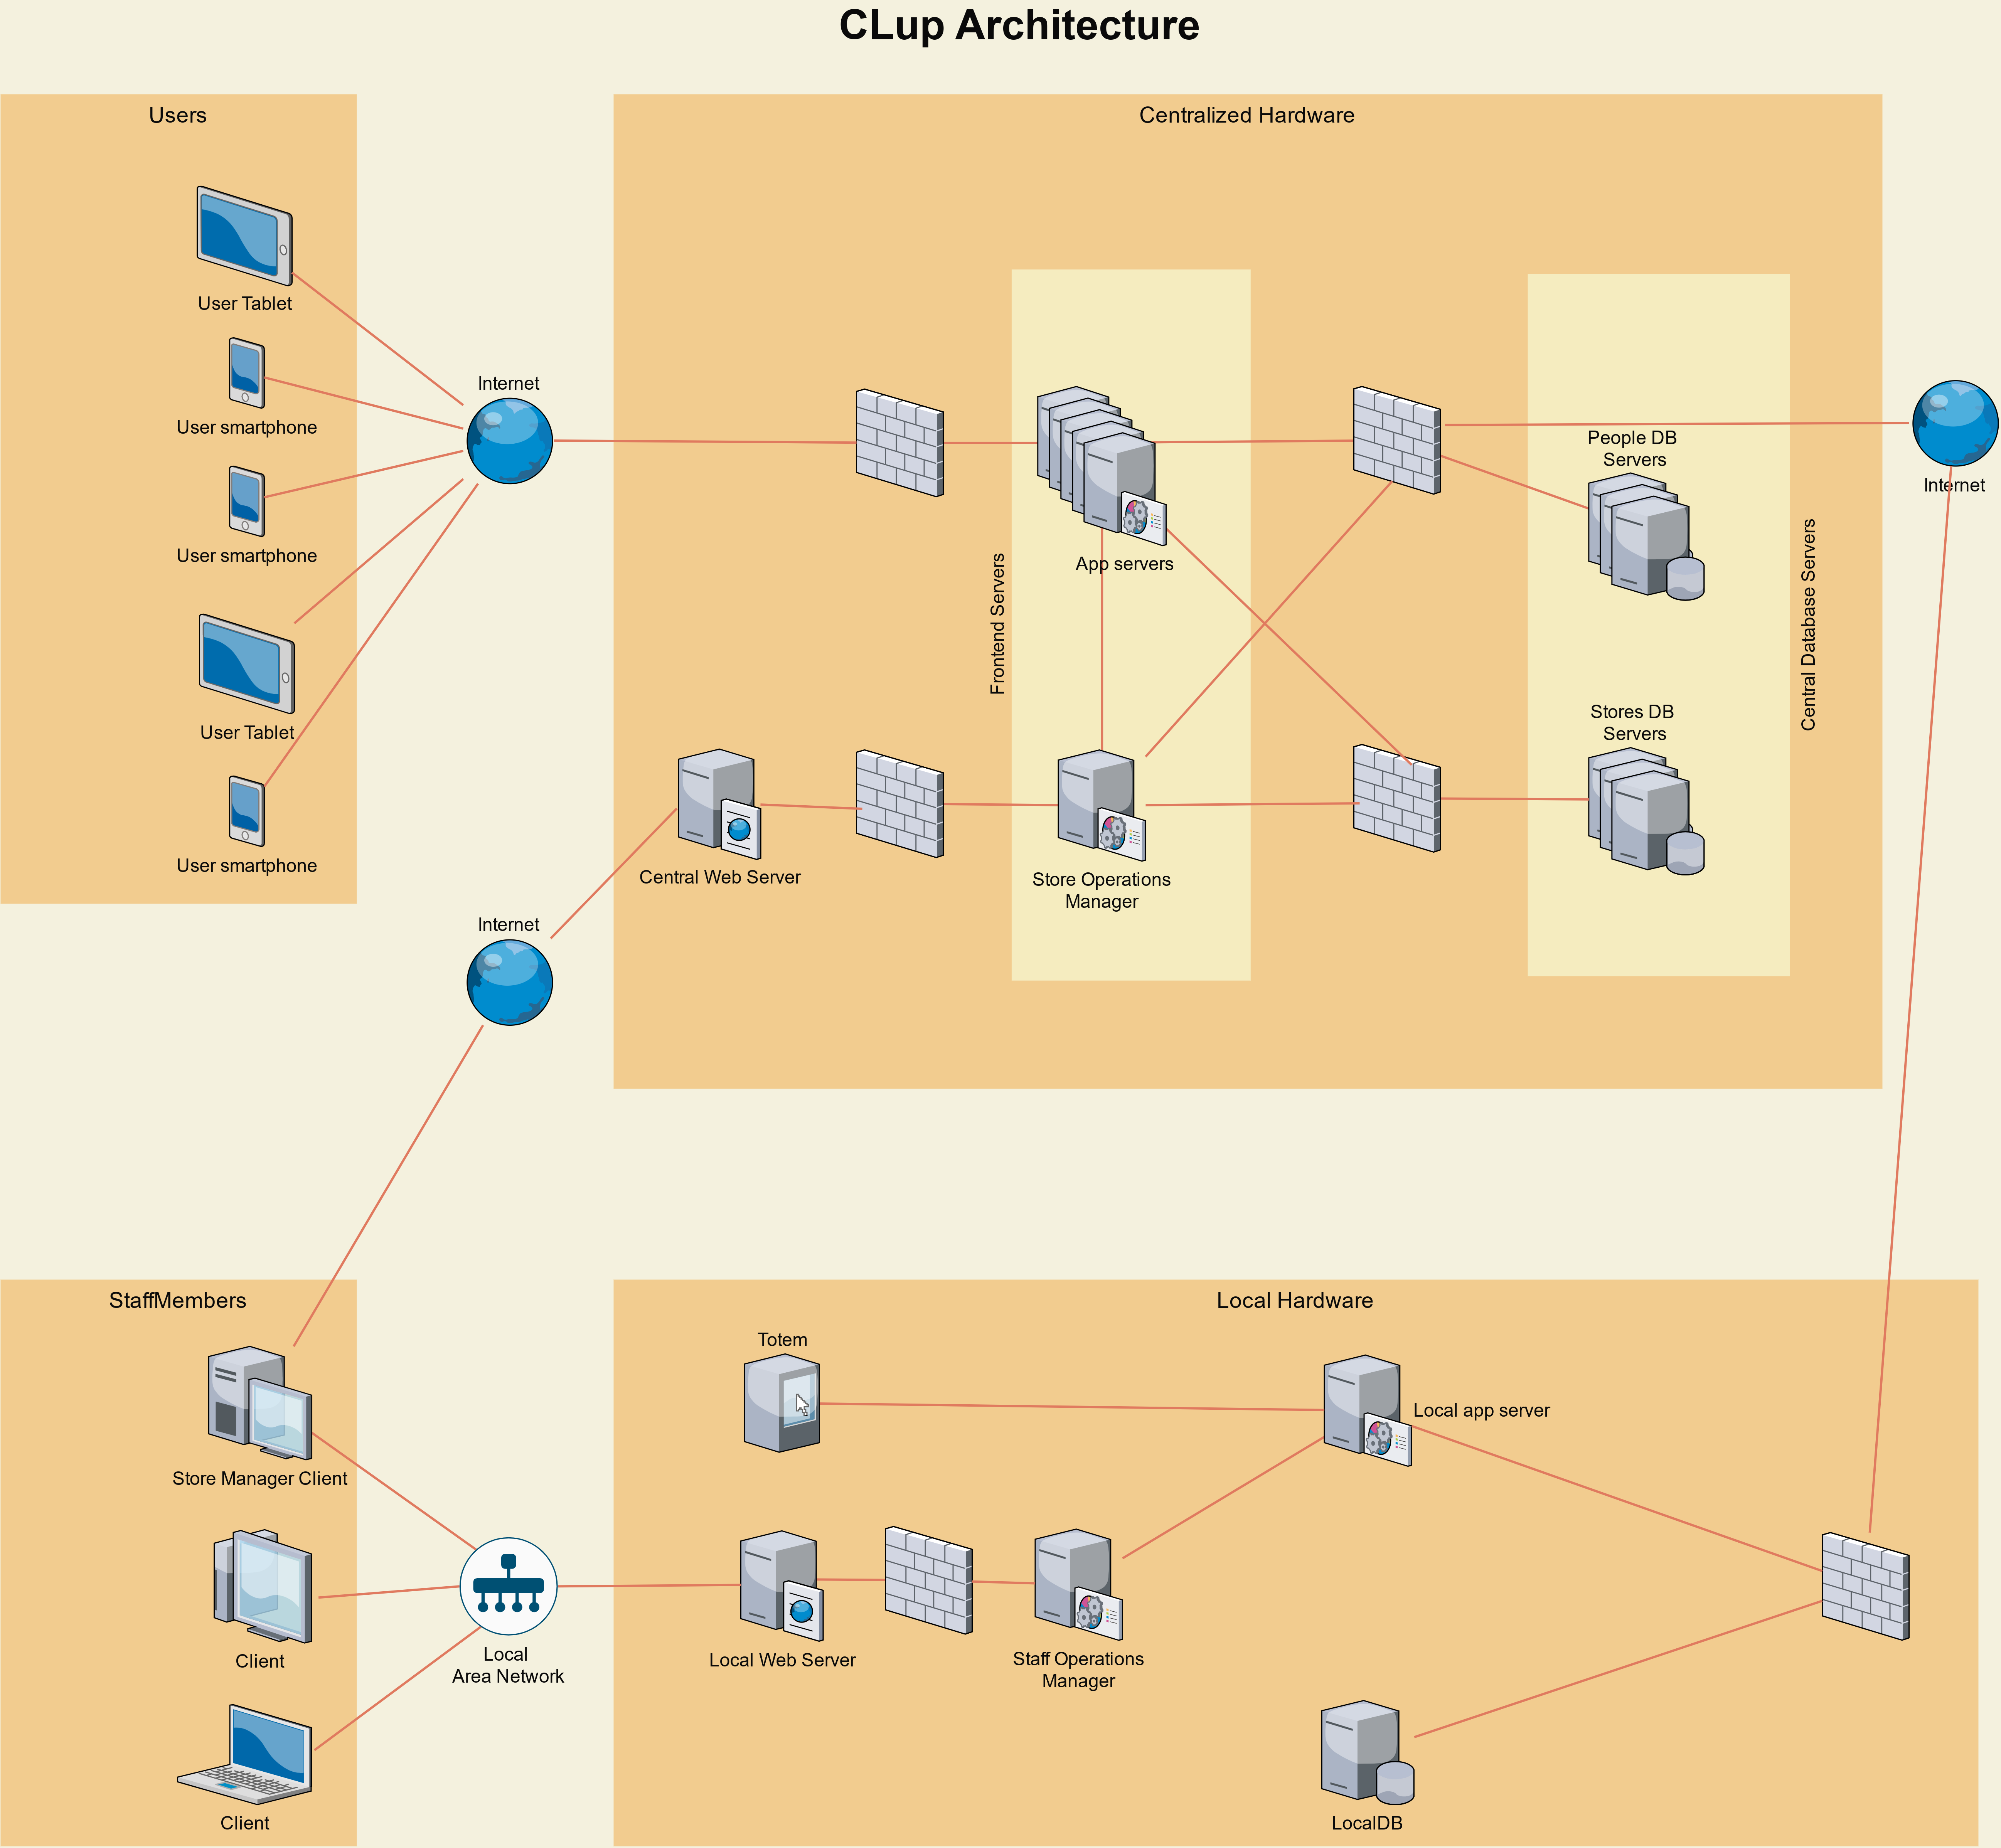
\includegraphics[width=\linewidth]{../Diagrams/Archtecture/Architecture_diagram.png}
	\caption{High-level architecture}
	\label{fig:HLArch}
\end{figure}

\subsection{Component view}

\begin{figure}[h!]
	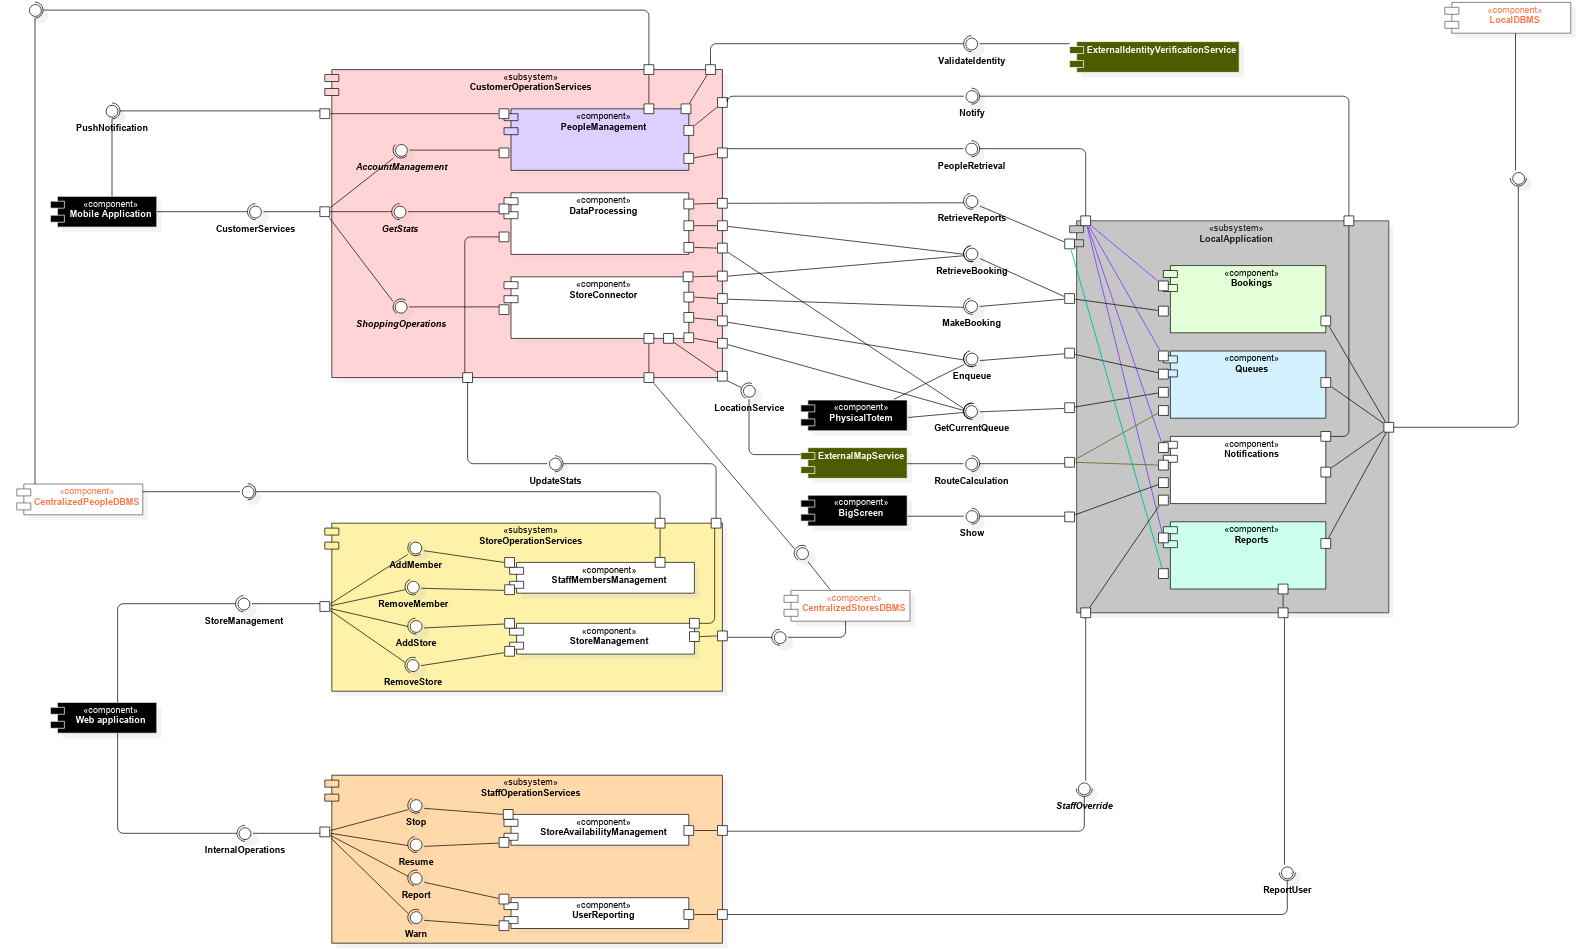
\includegraphics[width=\linewidth]{../Diagrams/ComponentDiagram.png}
	\caption{Component Diagram}
	\label{fig:CompDgm}
\end{figure}

In Figure \ref{fig:CompDgm} is represented the component diagram of the internal structure Application layer, showing how its components and subsystems interact. As previously said, the A layer contains Clup's functional business logic which drives the application’s core capabilities, it builds  a bridge between the presentation layer and the data layer. What follows is a brief description of every component and subsystem:
\begin{itemize}
	\item \textbf{Staff Operation Services}: This subsystem contains 2 components:
	\begin{itemize}
		\item \textbf{Store Availability Management}: This is the component responsible for both interruption and recovery of availability of a store to accept new virtually queued customers
		\item \textbf{User Reporting}: This component's function is to take note of customers bad behaviours 
	\end{itemize} 

	\item \textbf{Store Operation Services}: This subsystem contains 2 components:
	\begin{itemize}
		\item \textbf{Staff Members Management}: A subscribed store can grant access and credentials to CLup's store services through this component 
		\item \textbf{Store Management}: A store can enroll to CLup's network through this component
	\end{itemize} 

	\item \textbf{Customer Operation Services}: This subsystem has 2 subcomponents
	\begin{itemize}
		\item \textbf{People Management}: This component is responsible for customers subscription, login t CLup and, thanks to the association device-person, notifications by CLup and Supermarkets
		\item \textbf{Data Processing}: As says the name, the Data Processing component takes care of data about availability of stores, time slots and queues status. It also evaluate time slots, days and store crowdness level and infer better solutions.
		\item \textbf{Store Connector}:TODO
	\end{itemize}

	\item \textbf{Local Application }:
	\begin{itemize}
		\item \textbf{Bookings}: This component makes possible booking an entrance, it takes care of the logic of the booking procedure and retrieves information of a previously made reservation
		\item \textbf{Queues}: This is the component responsible for the basic function of CLup, it has read-write access to stores queues and allows also to block and unblock them
		\item \textbf{Notifications}: Here is were all kind of users notifications are generated
		\item \textbf{Reports}: This is the component that instead generate bad behaviours reports
	\end{itemize}
	\item \textbf{External Map Services}: This is the component that provides the map interface
	\item \textbf{Physical Totem}: This component is a simplified version of the mobile app, it has only what is needed to perform the basic function.
\end{itemize}

\subsection{Deployment view}
\subsection{Runtime view}
\begin{figure}[H]
	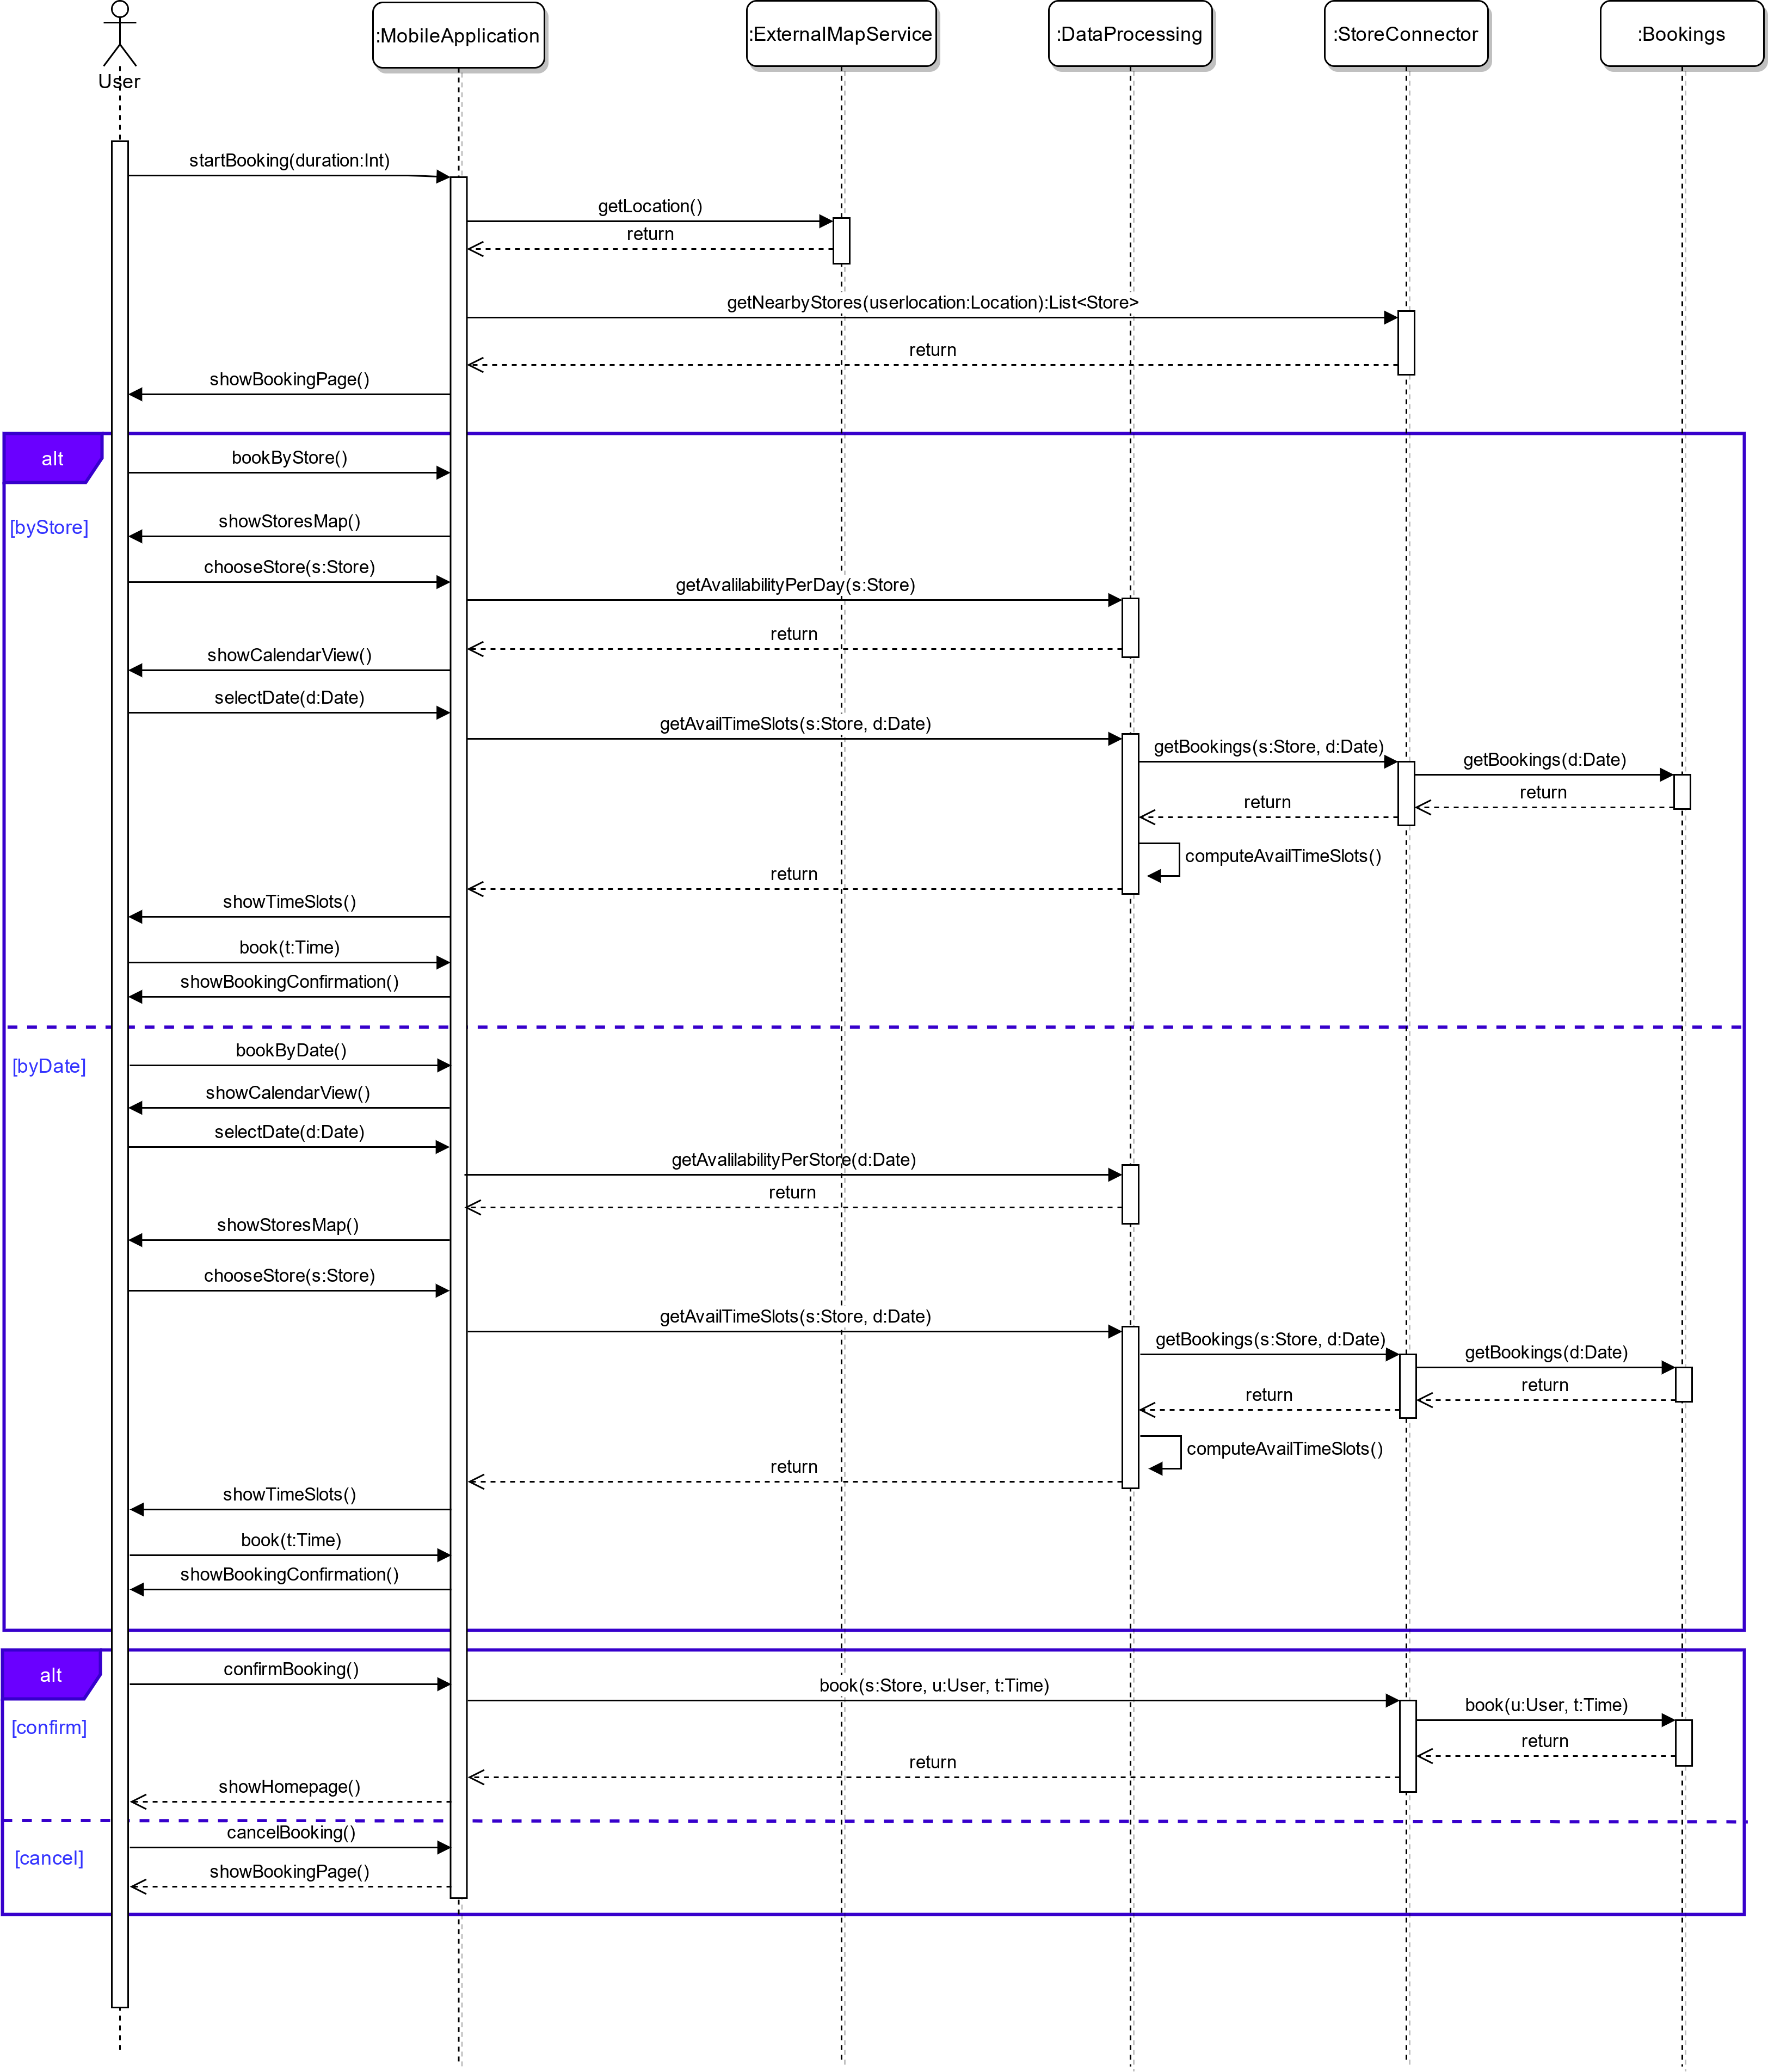
\includegraphics[width=\linewidth]{../Diagrams/Sequence/sequence_customer_book.png}
	\caption{Sequence Diagram: Customer Booking}
	\label{fig:sCusBook}
\end{figure}

\begin{figure}[H]
	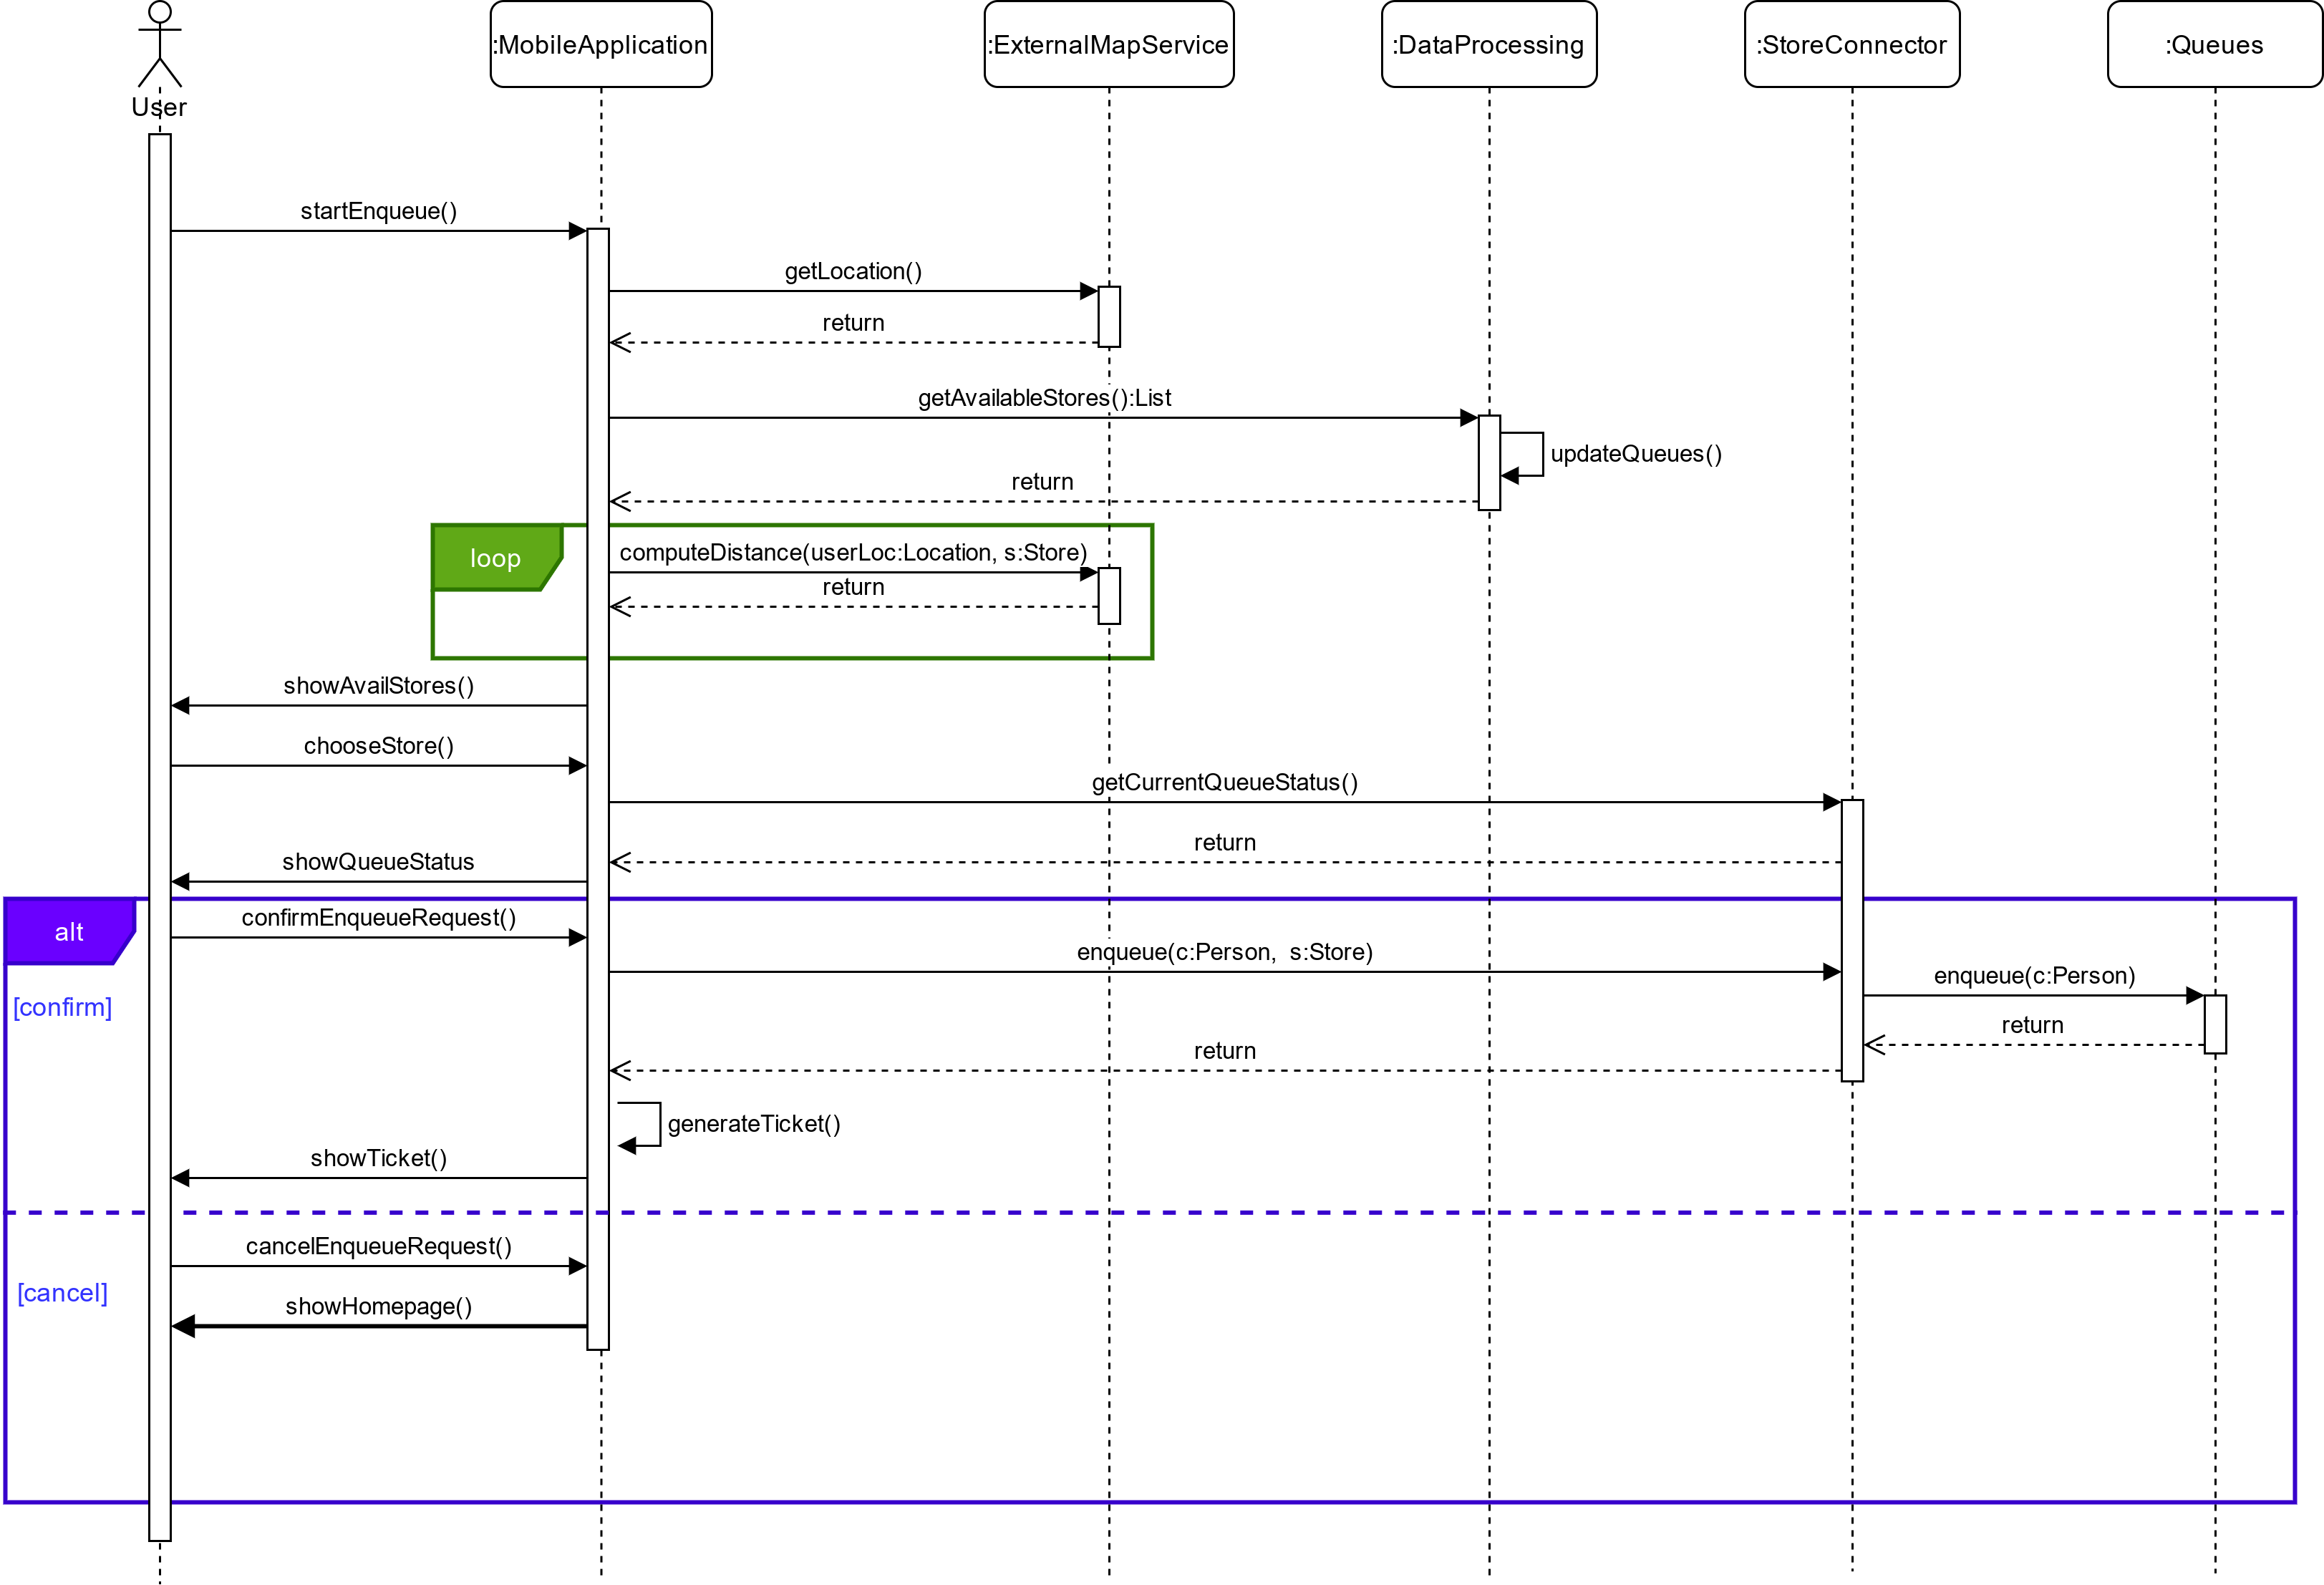
\includegraphics[width=\linewidth]{../Diagrams/Sequence/sequence_customer_enqueue.png}
	\caption{Sequence Diagram: Customer Enqueue}
	\label{fig:sCusEnq}
\end{figure}

\begin{figure}[H]
	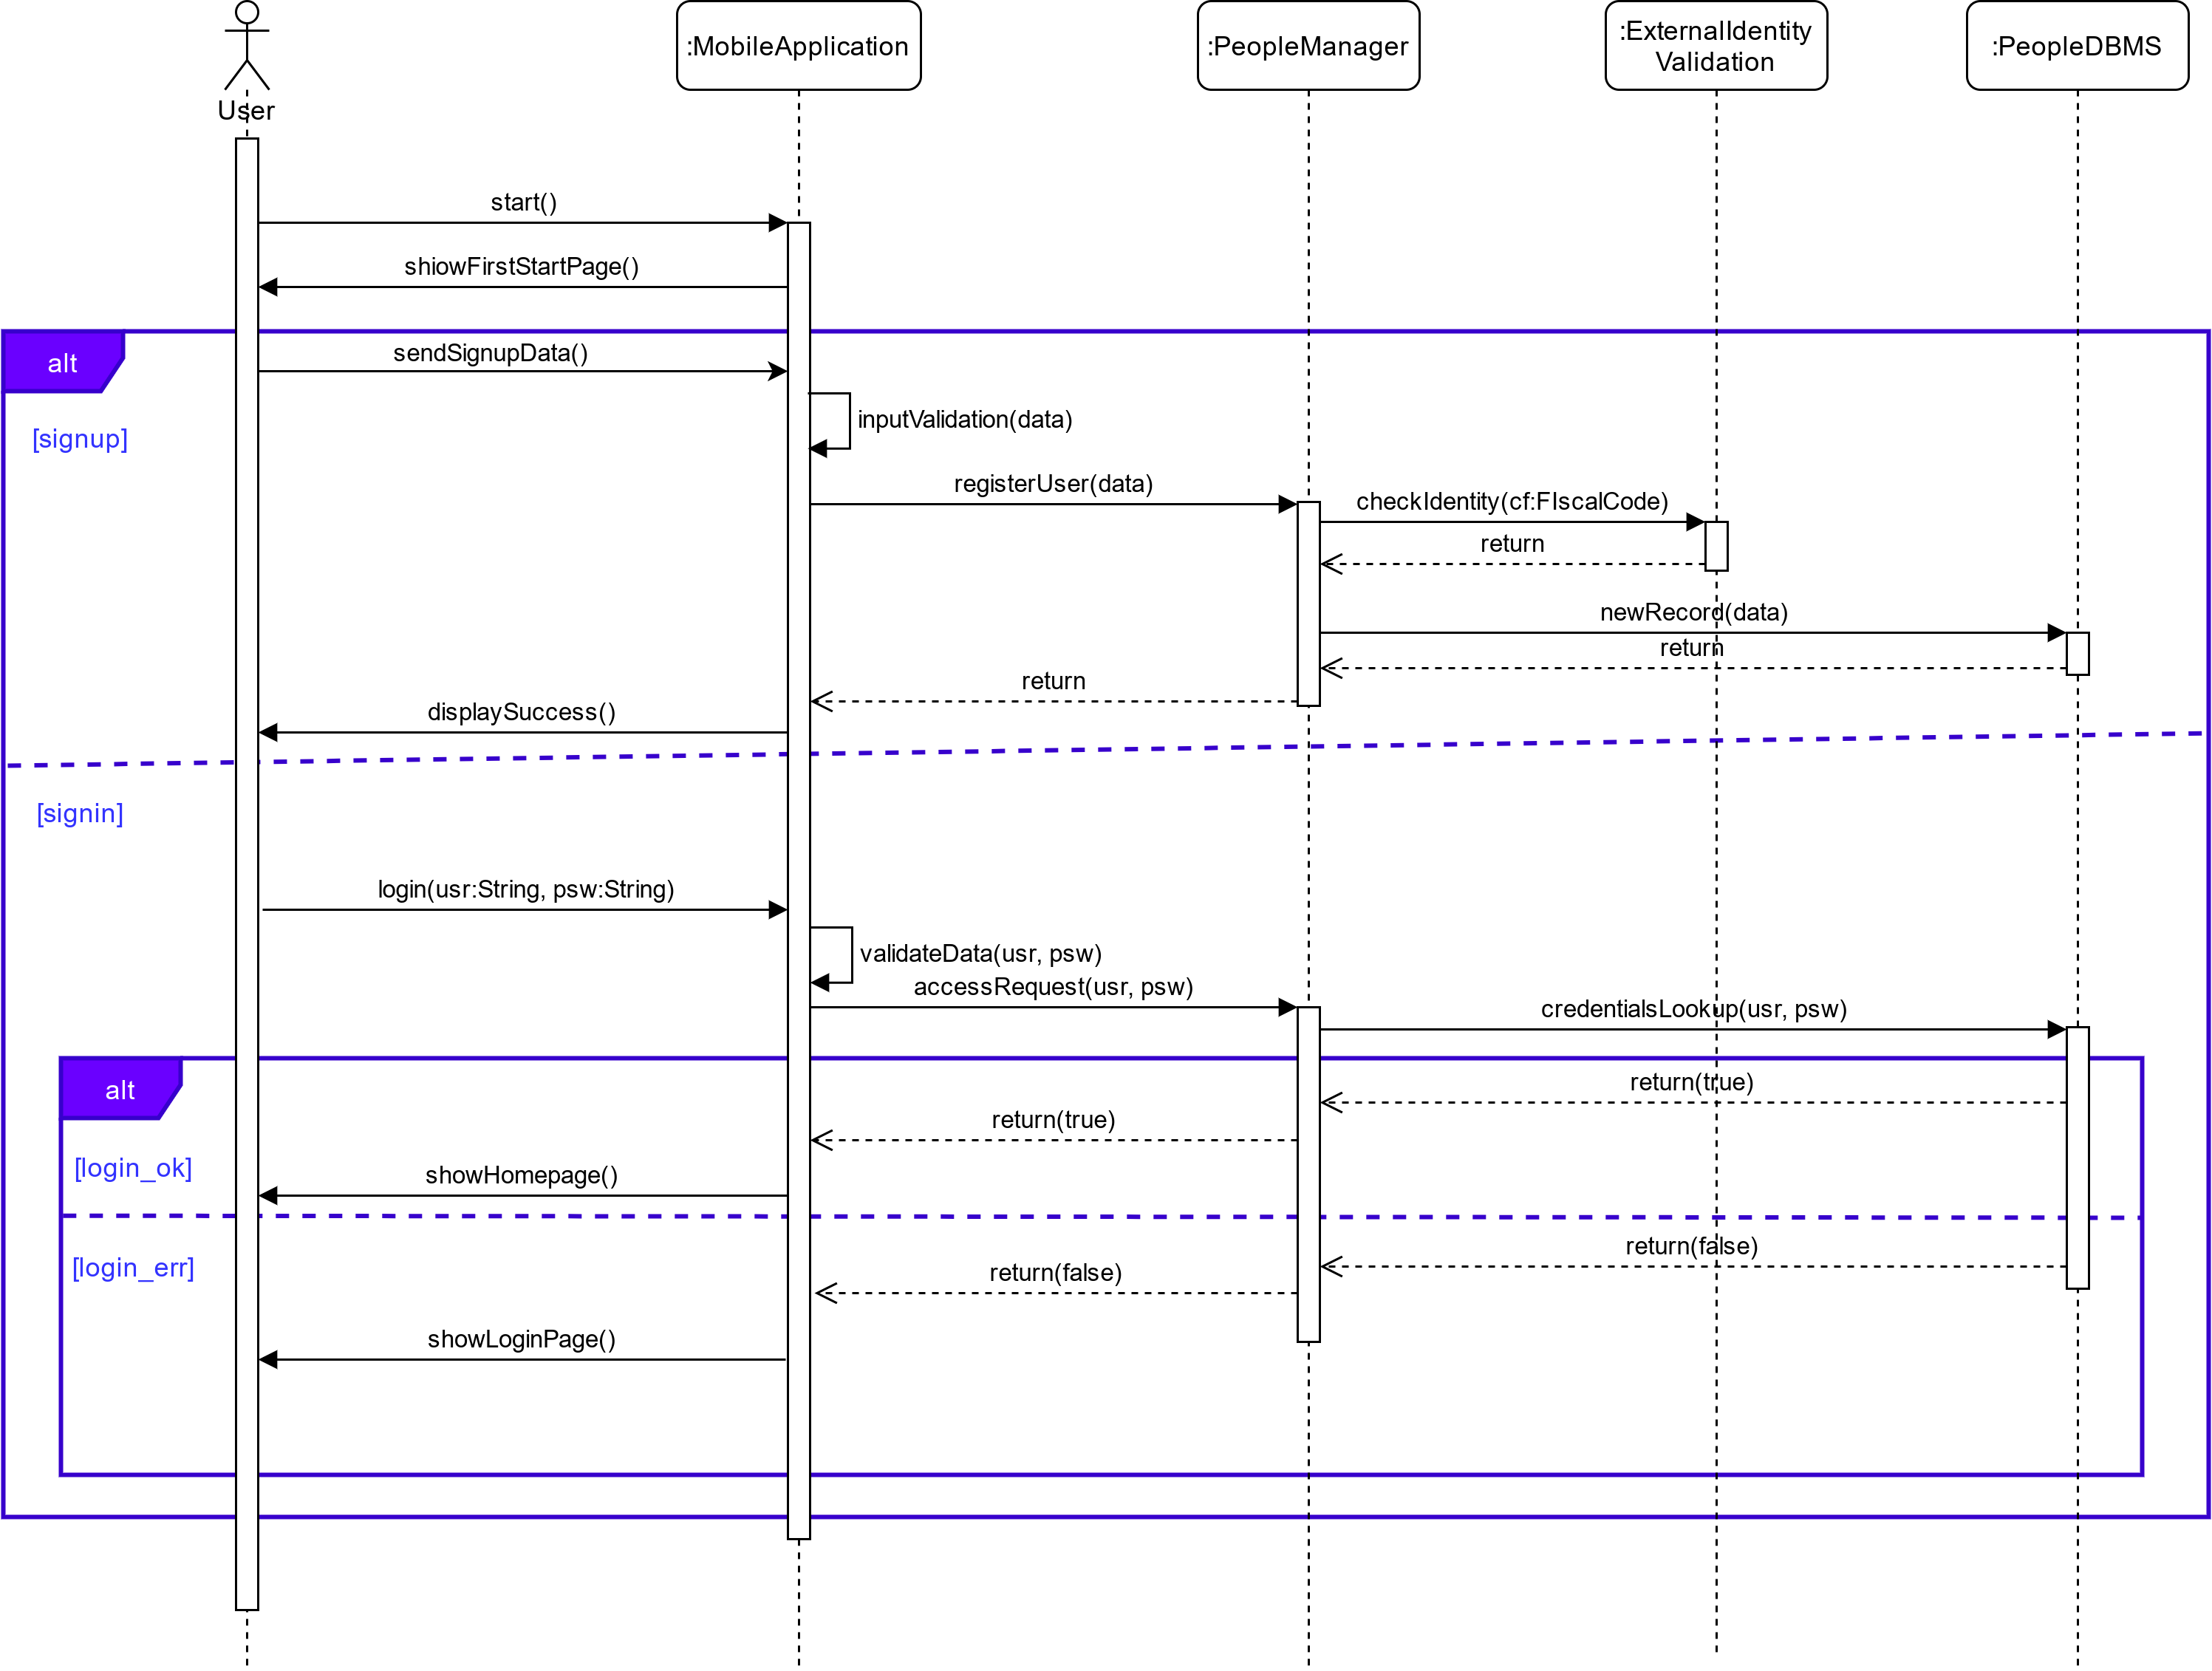
\includegraphics[width=\linewidth]{../Diagrams/Sequence/sequence_customer_signup.png}
	\caption{Sequence Diagram: Customer Signup}
	\label{fig:sCusSign}
\end{figure}

\begin{figure}[H]
	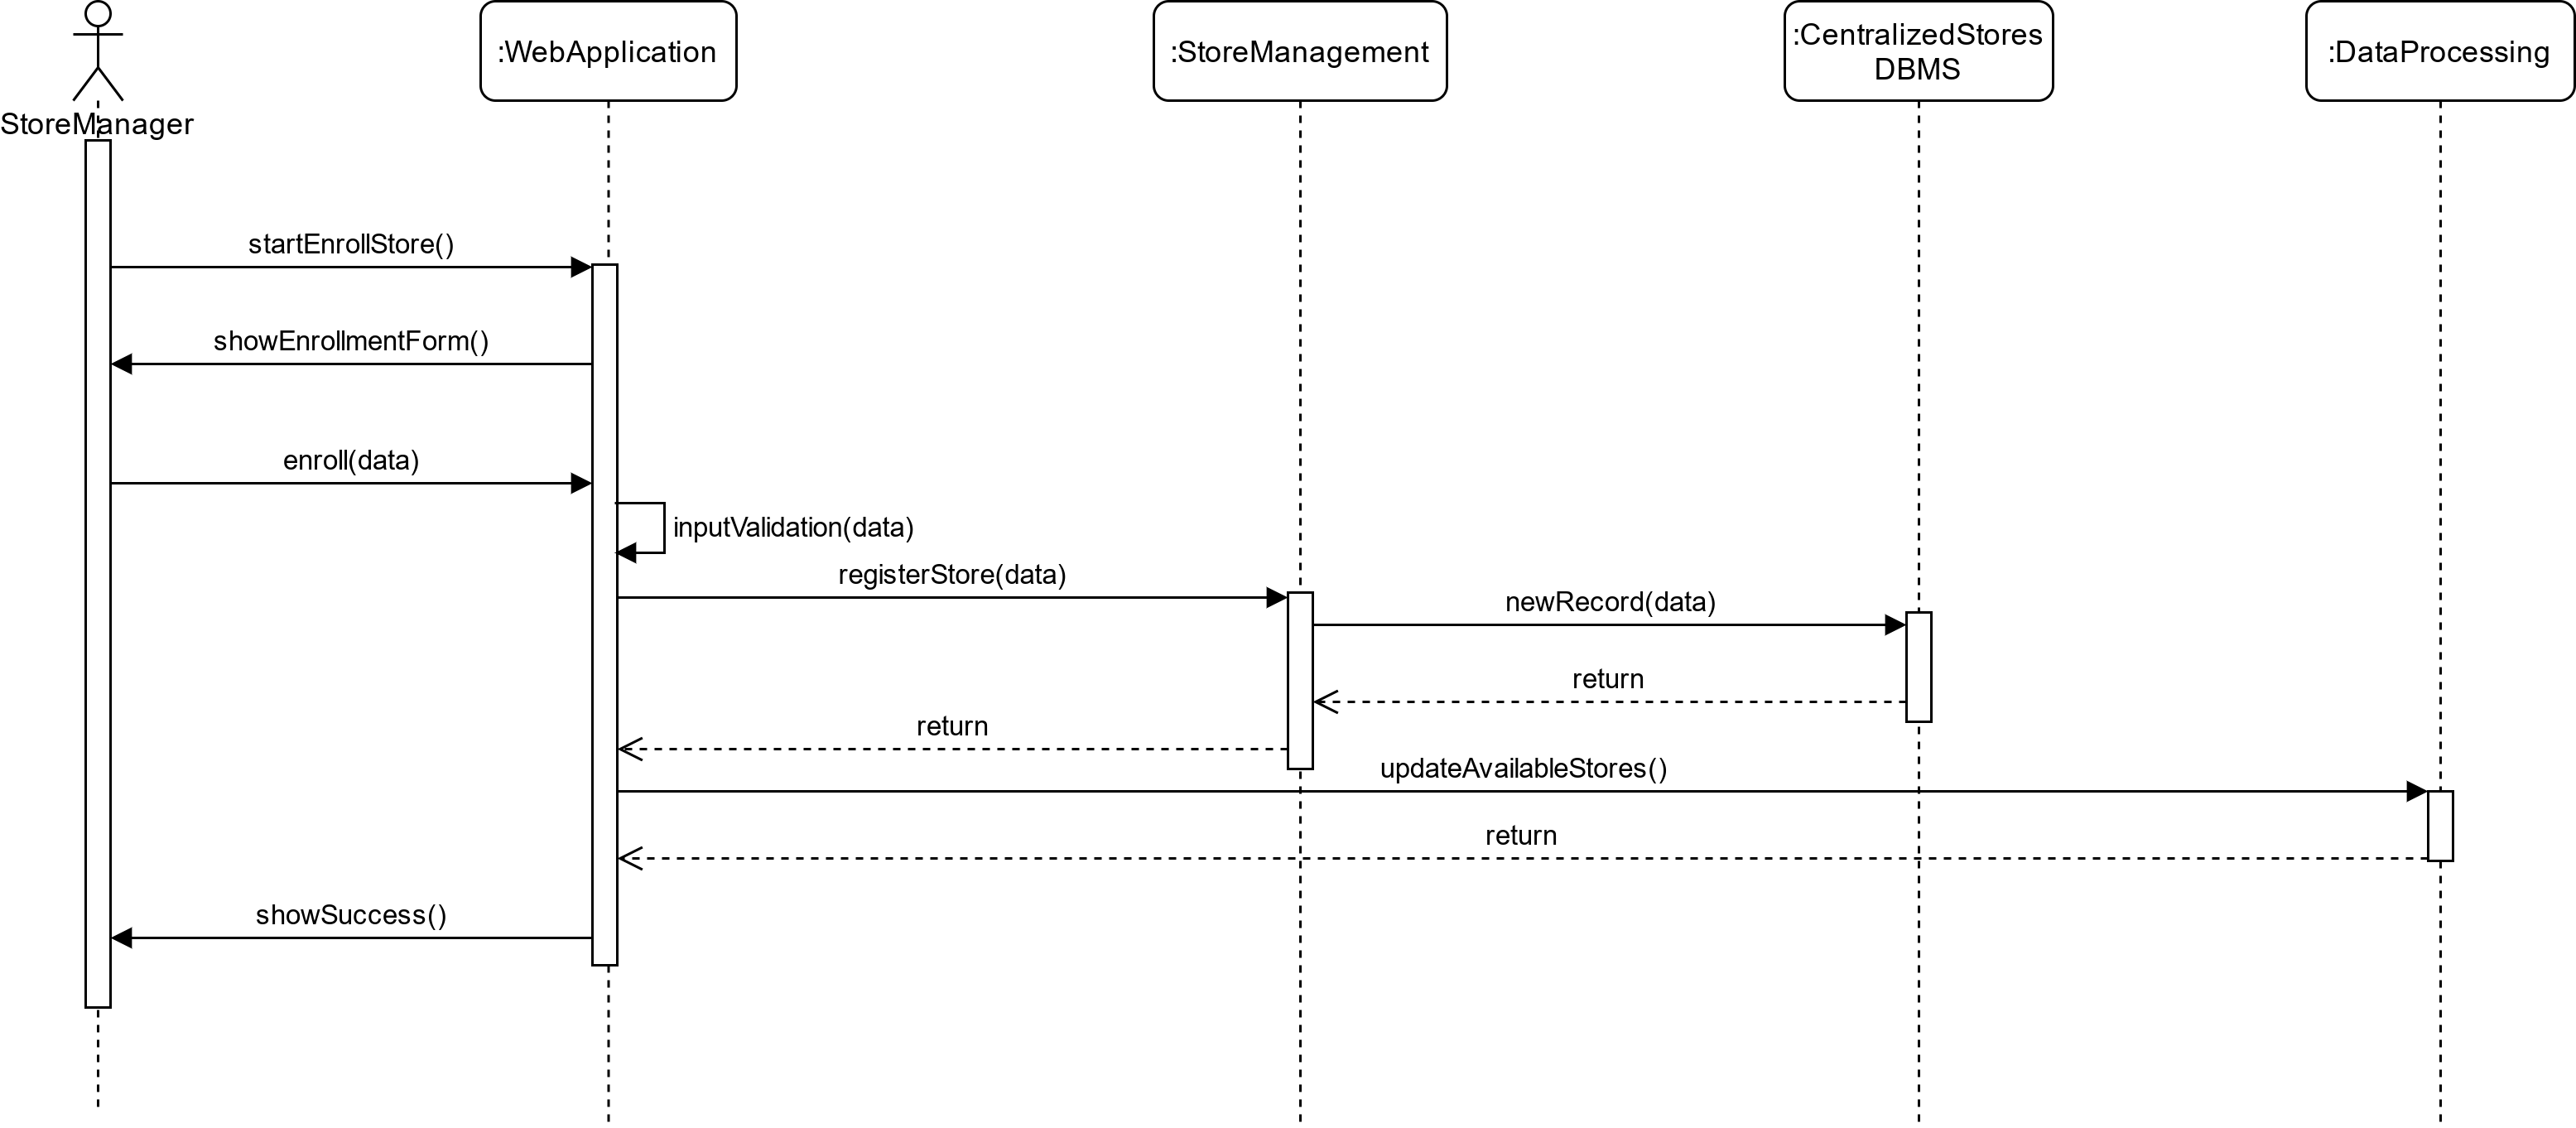
\includegraphics[width=\linewidth]{../Diagrams/Sequence/sequence_store_enroll.png}
	\caption{Sequence Diagram: Store Enroll}
	\label{fig:sStoreEn}
\end{figure}

\begin{figure}[H]
	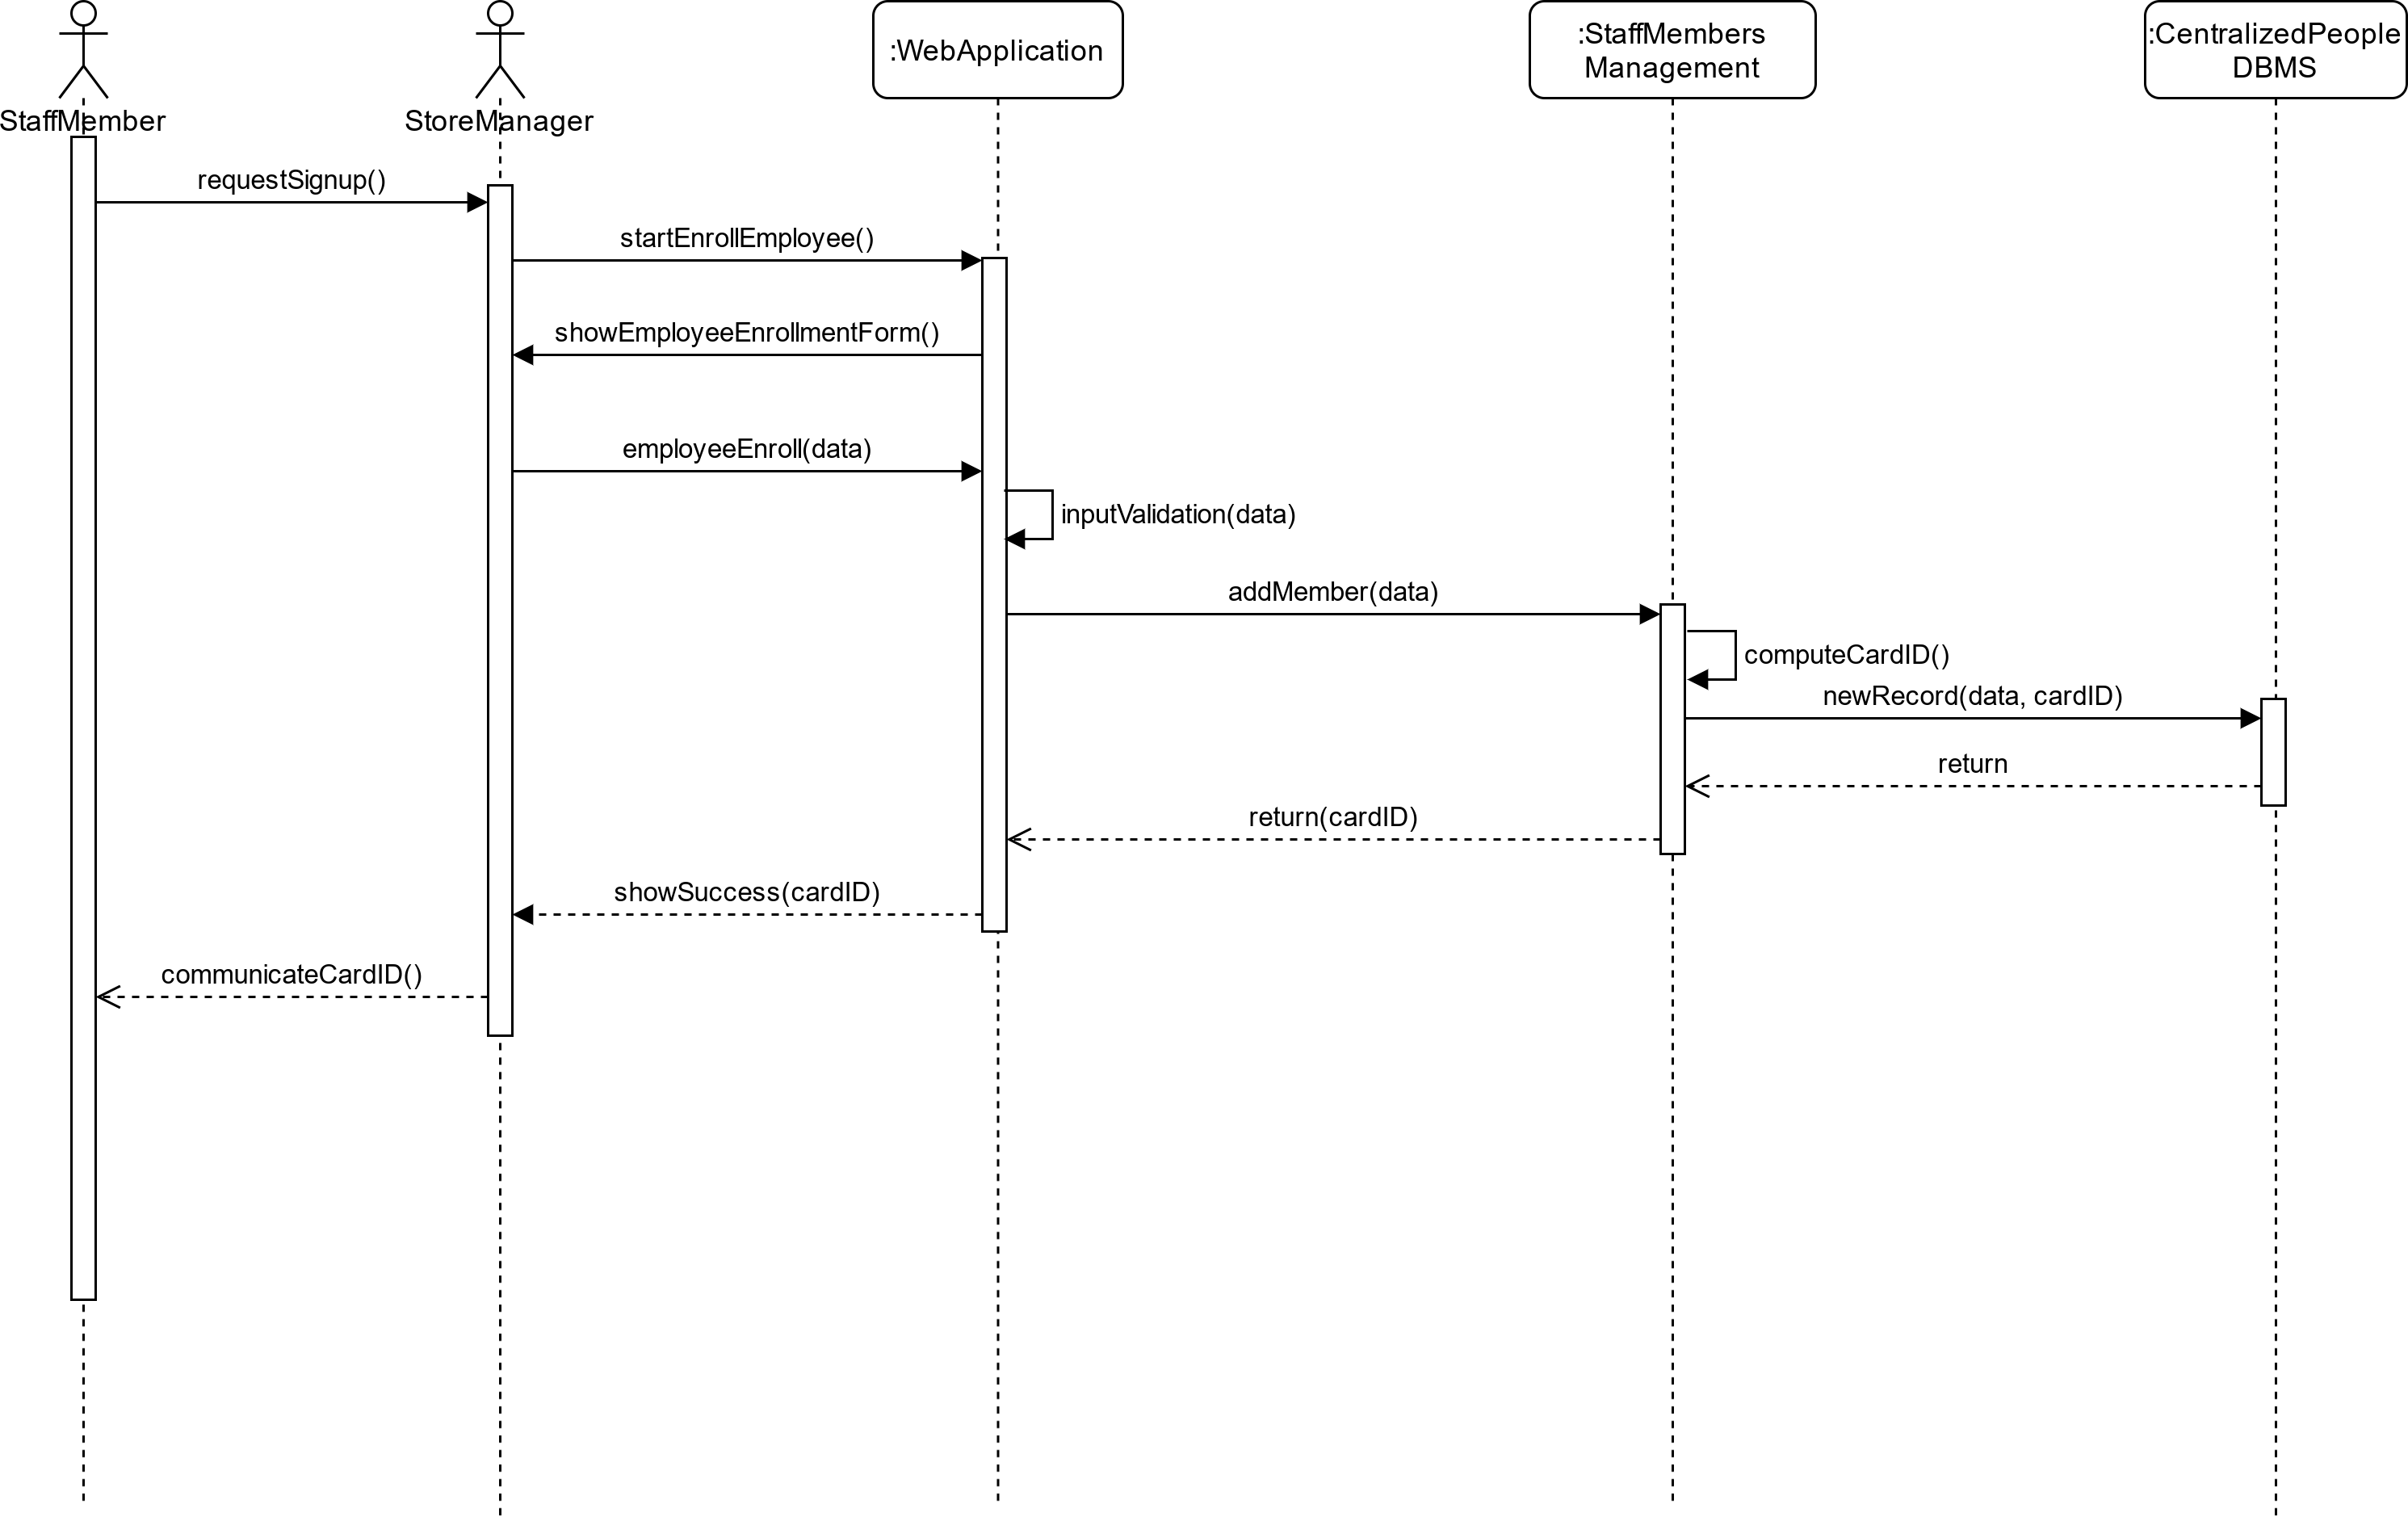
\includegraphics[width=\linewidth]{../Diagrams/Sequence/sequence_staff_enroll.png}
	\caption{Sequence Diagram: Staff Enroll}
	\label{fig:sStaffEn}
\end{figure}
\begin{figure}[H]
	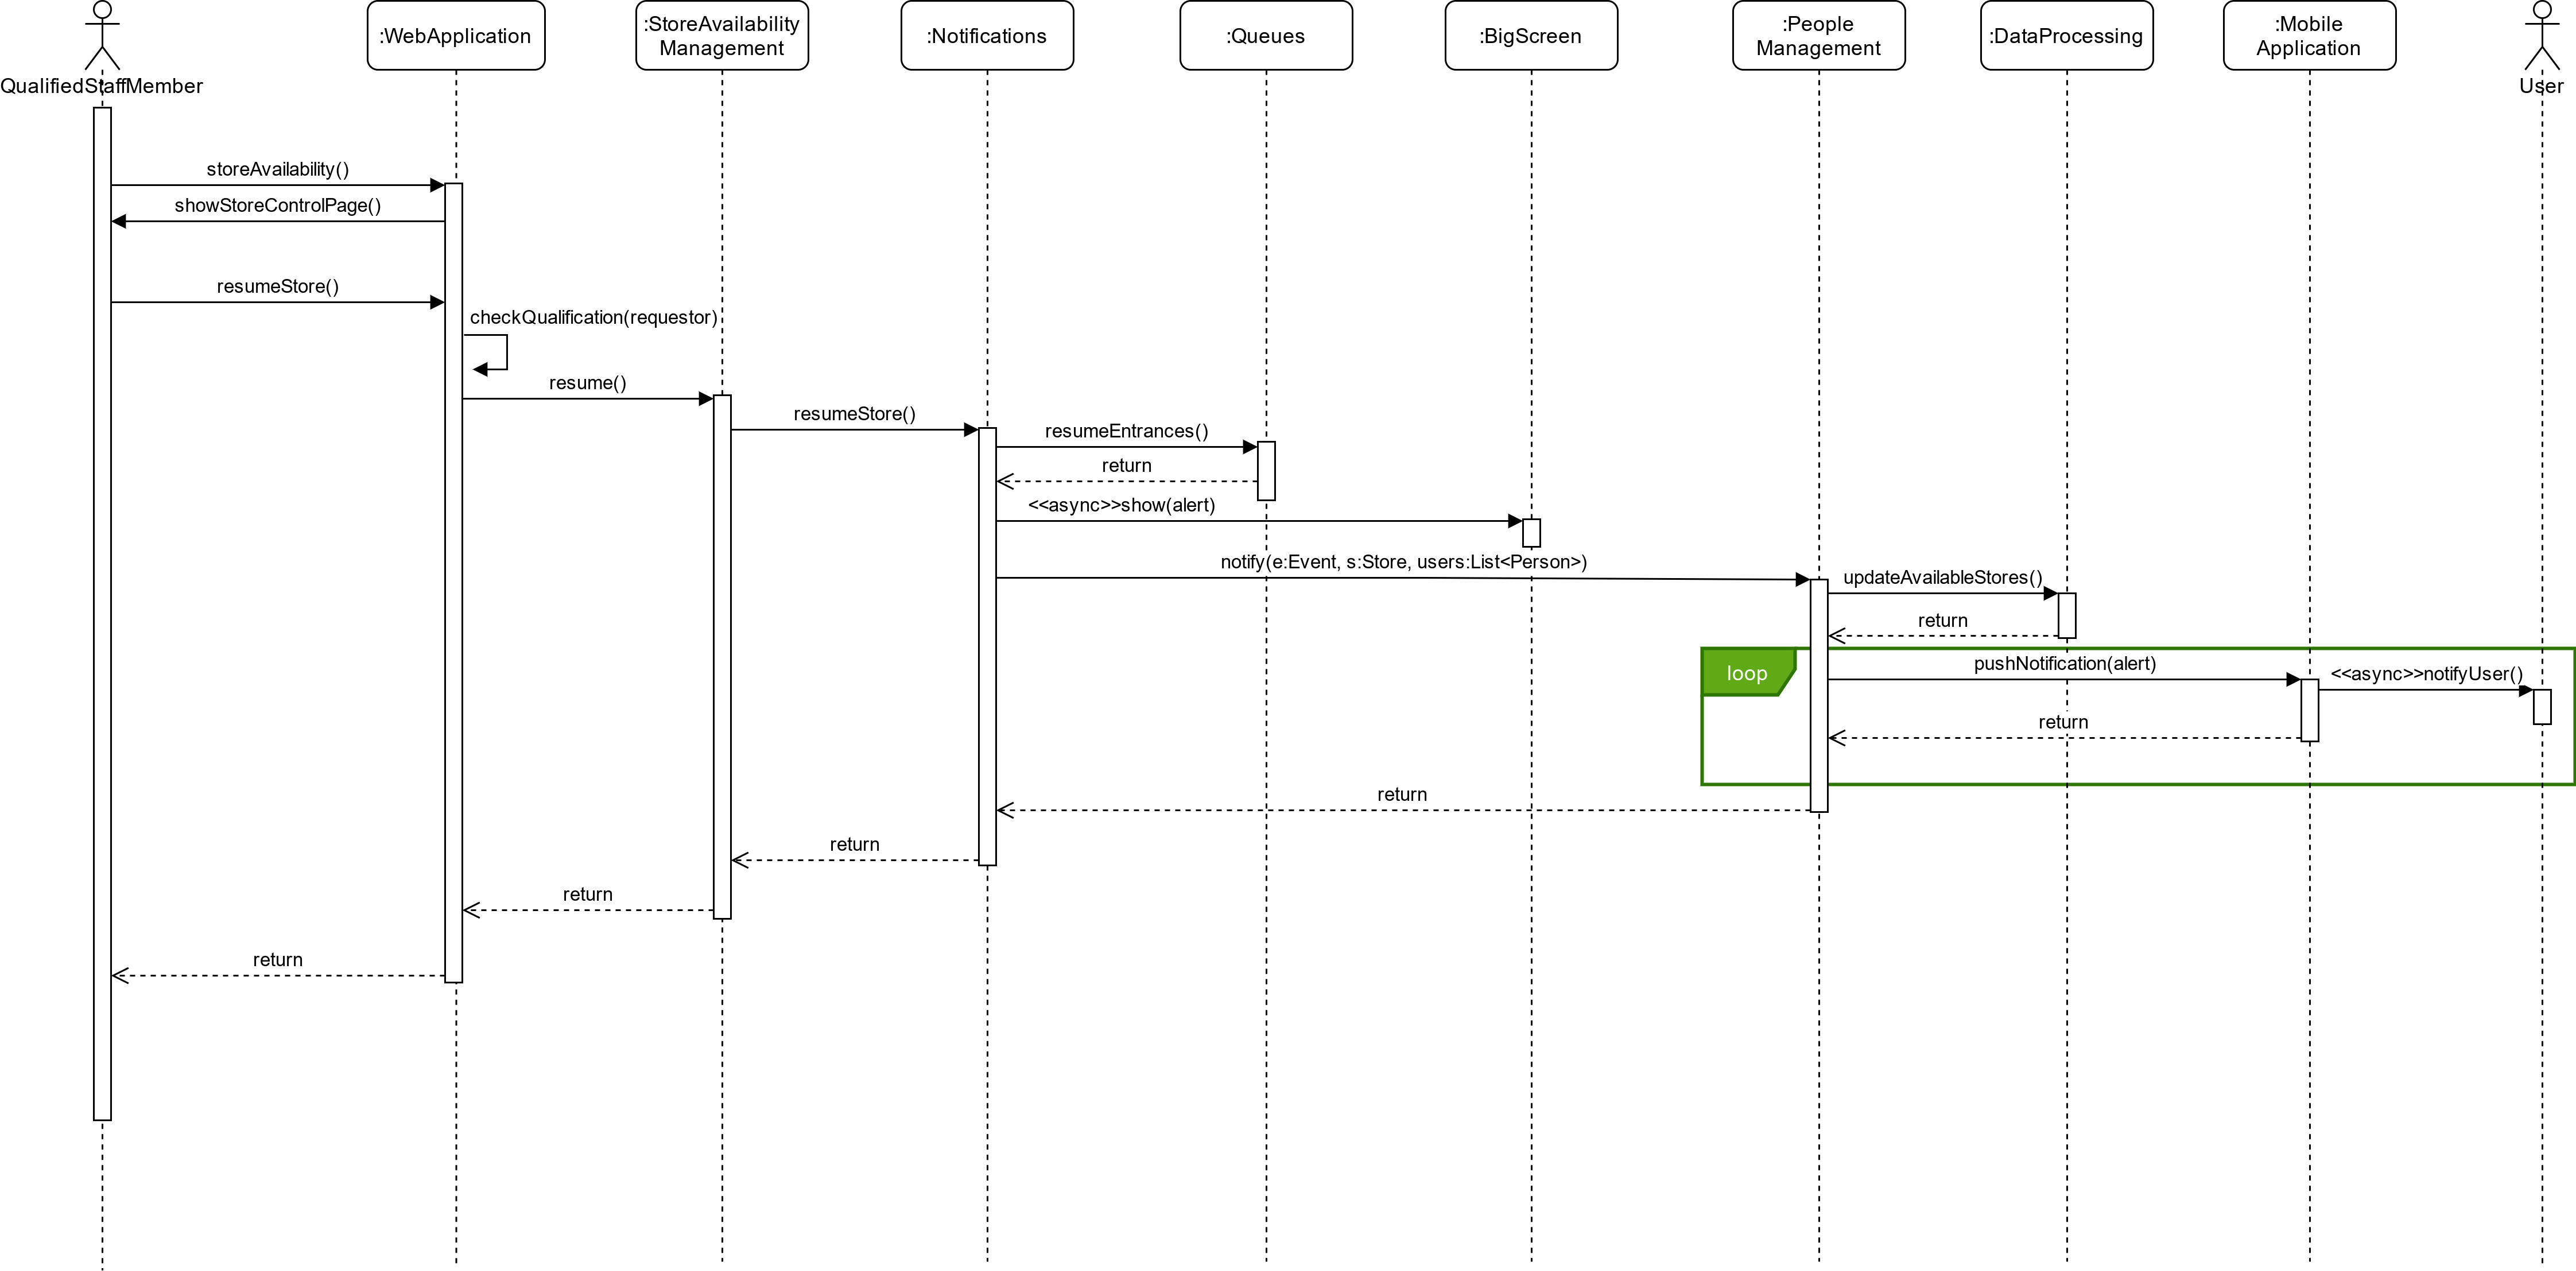
\includegraphics[width=\linewidth]{../Diagrams/Sequence/sequence_store_resume.png}
	\caption{Sequence Diagram: Store Resume}
	\label{fig:sStoreRes}
\end{figure}
\begin{figure}[H]
	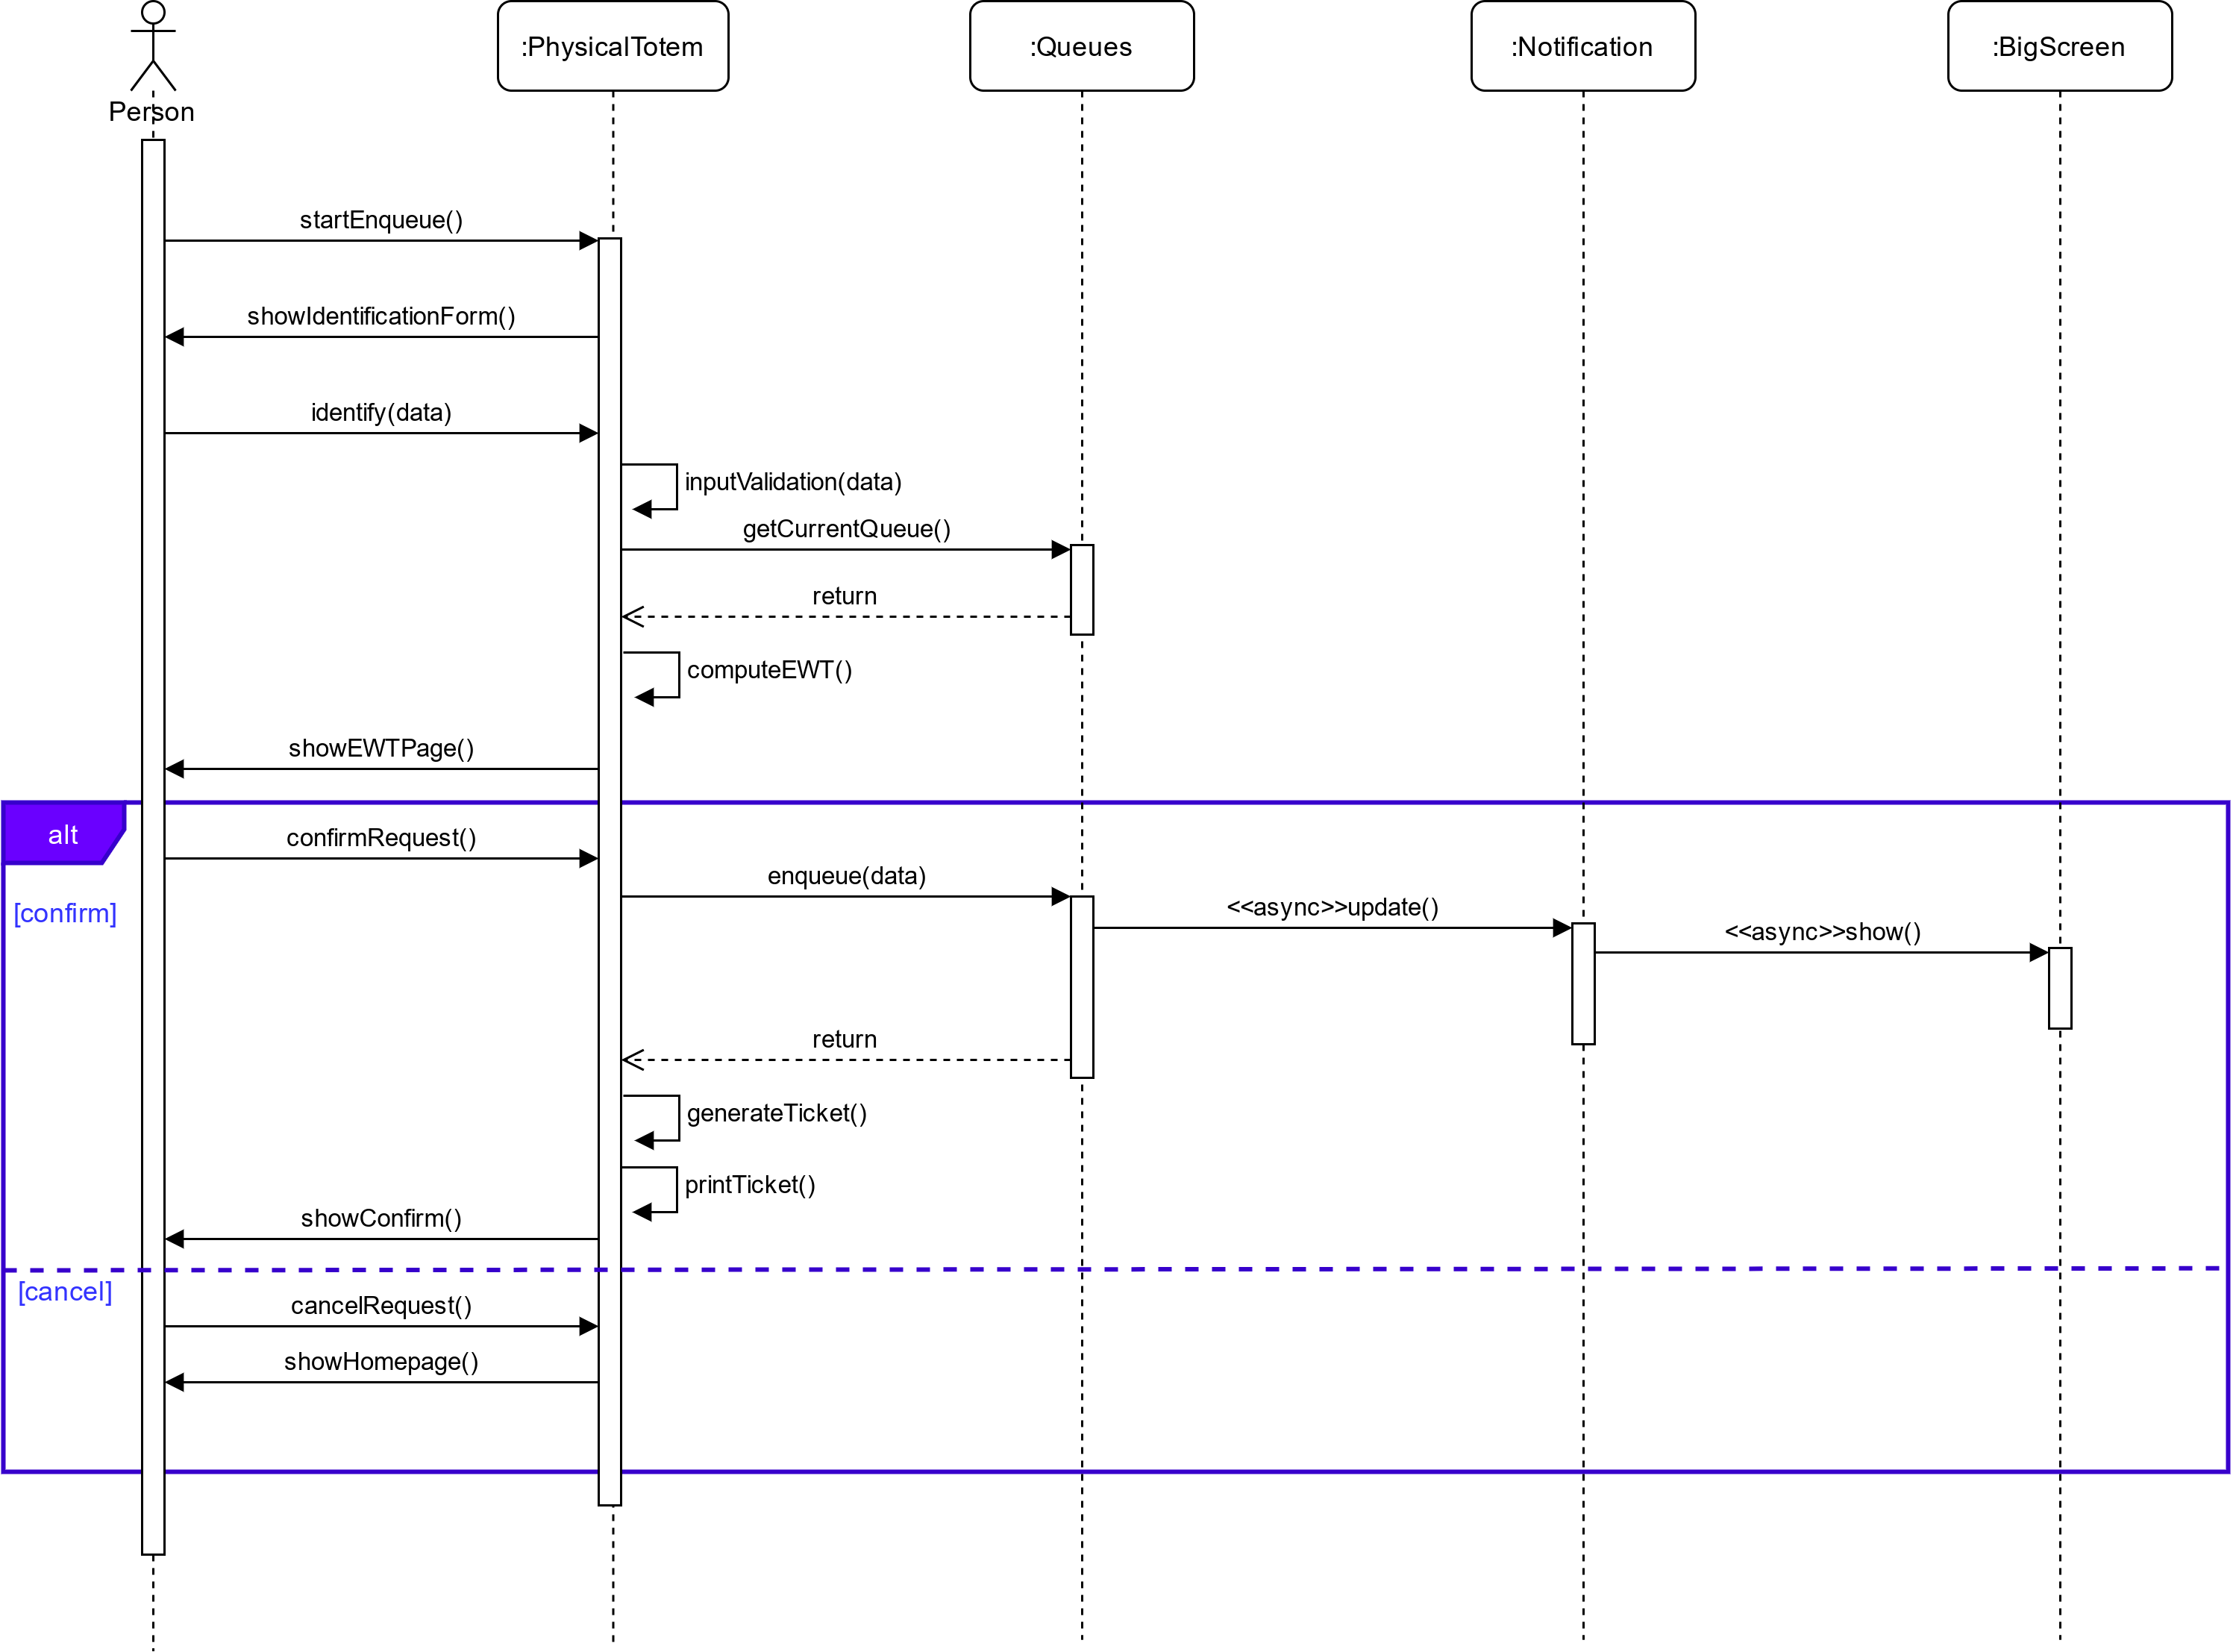
\includegraphics[width=\linewidth]{../Diagrams/Sequence/sequence_totem_enqueue.png}
	\caption{Sequence Diagram: Totem Enqueue}
	\label{fig:sTotemEnq}
\end{figure}

\begin{figure}[H]
	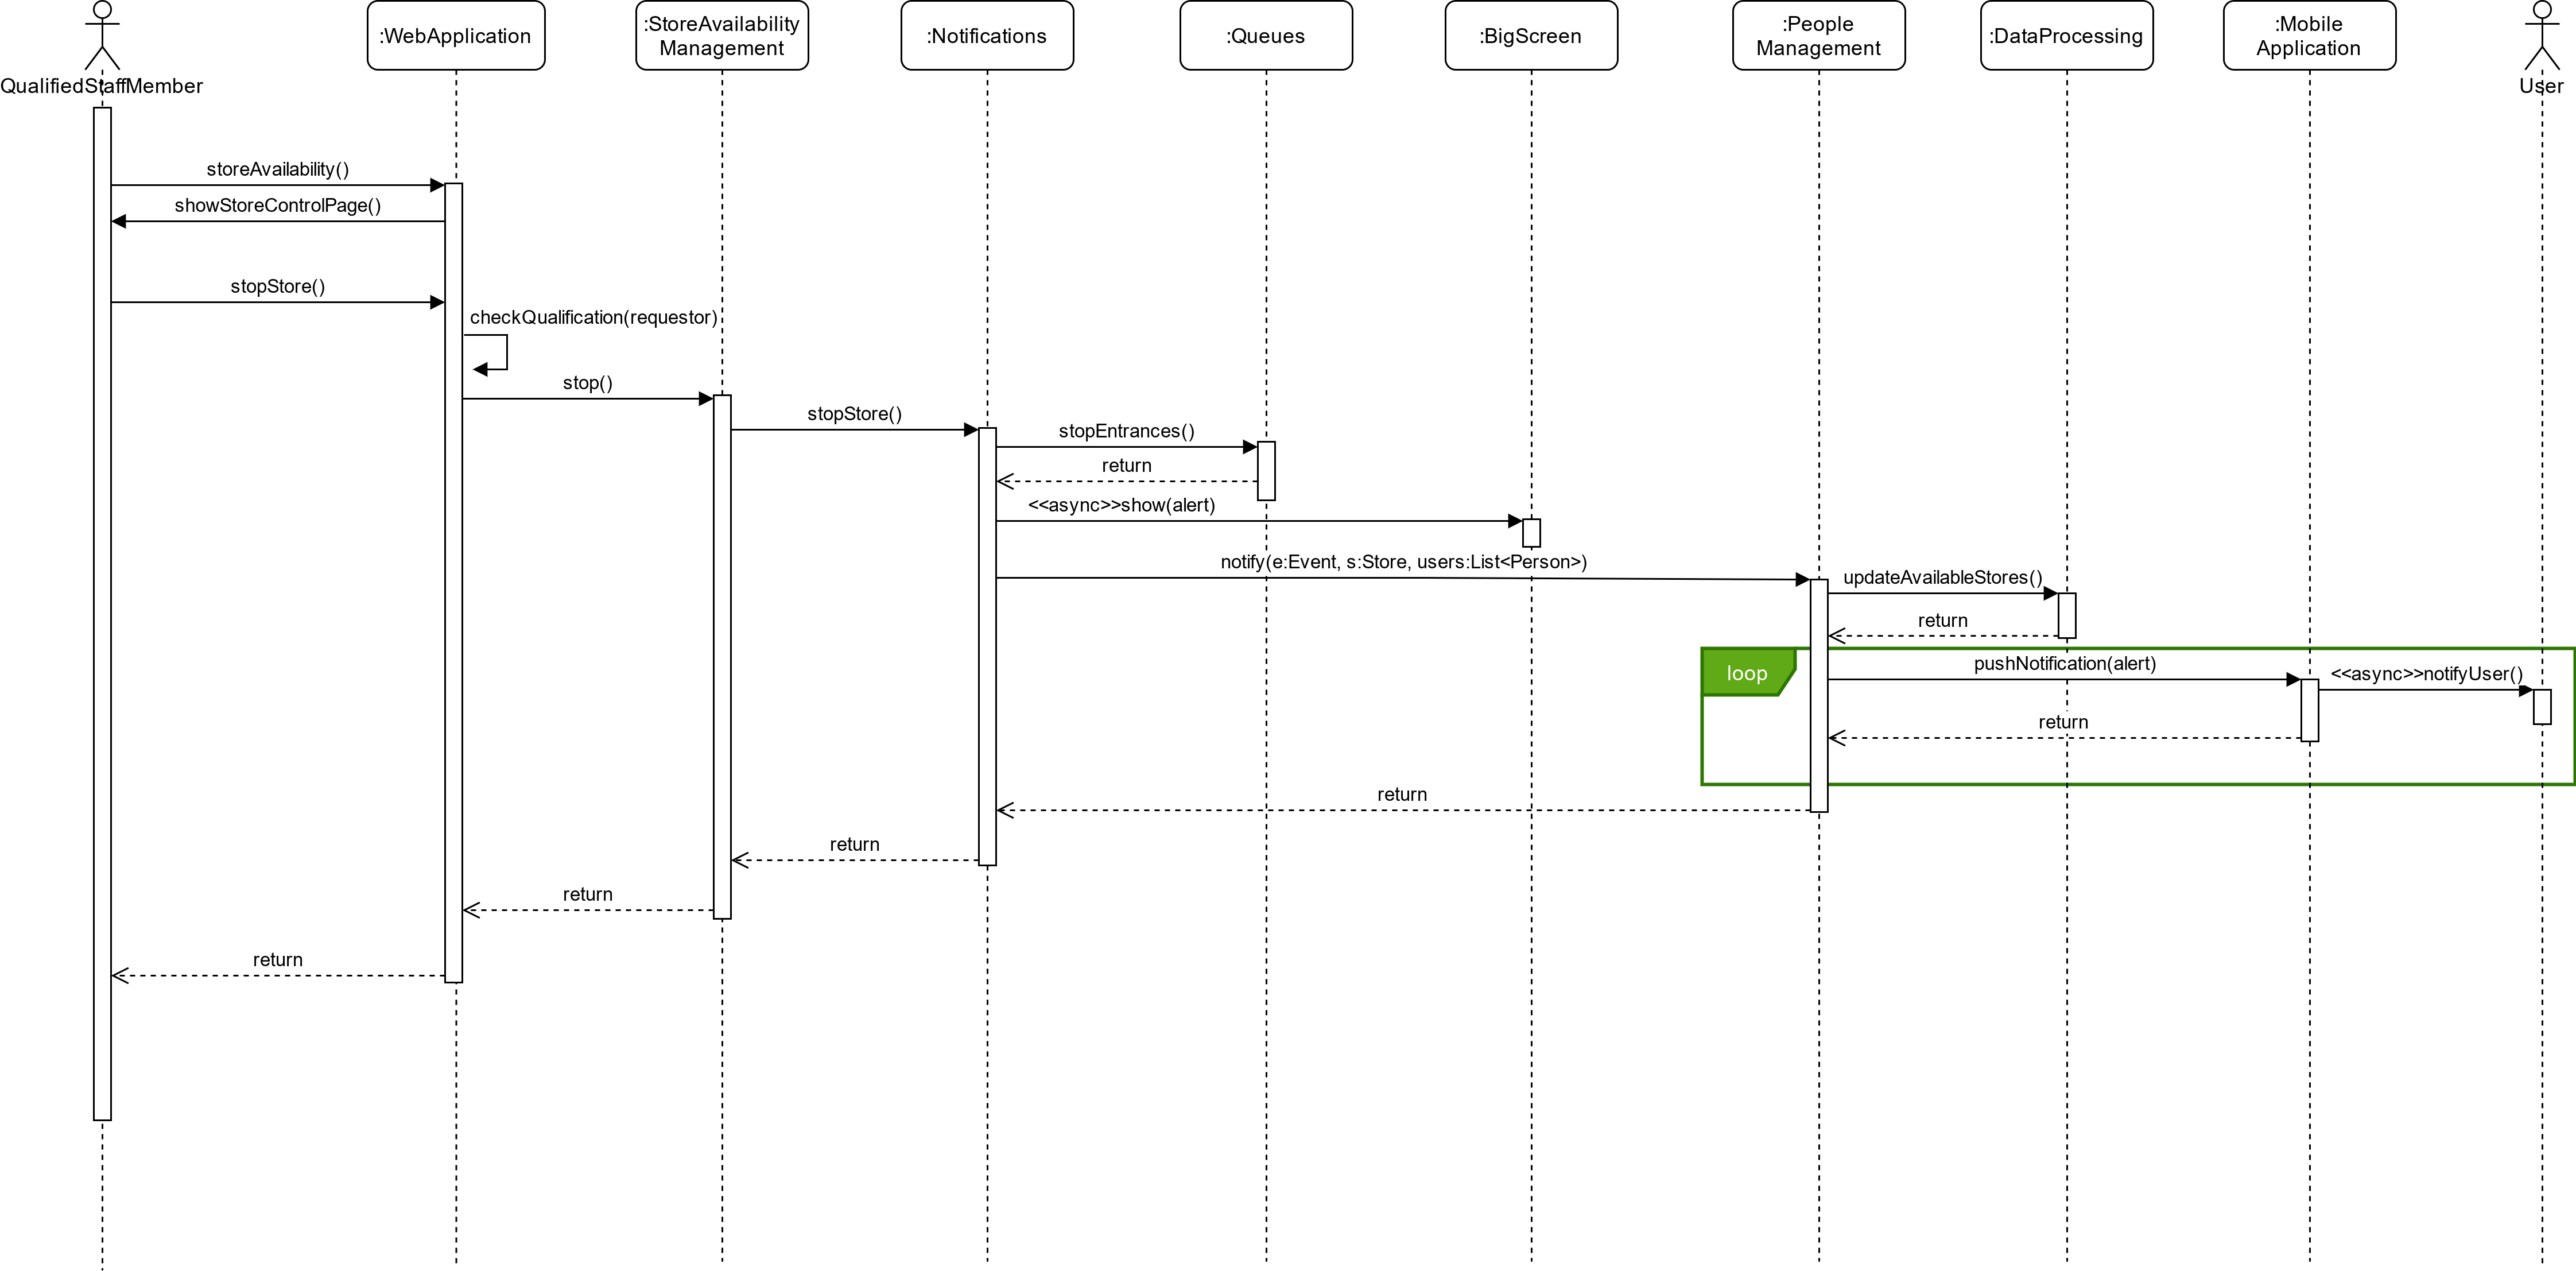
\includegraphics[width=\linewidth]{../Diagrams/Sequence/sequence_store_override.png}
	\caption{Sequence Diagram: Store Override}
	\label{fig:sStoreOver}
\end{figure}

\begin{figure}[H]
	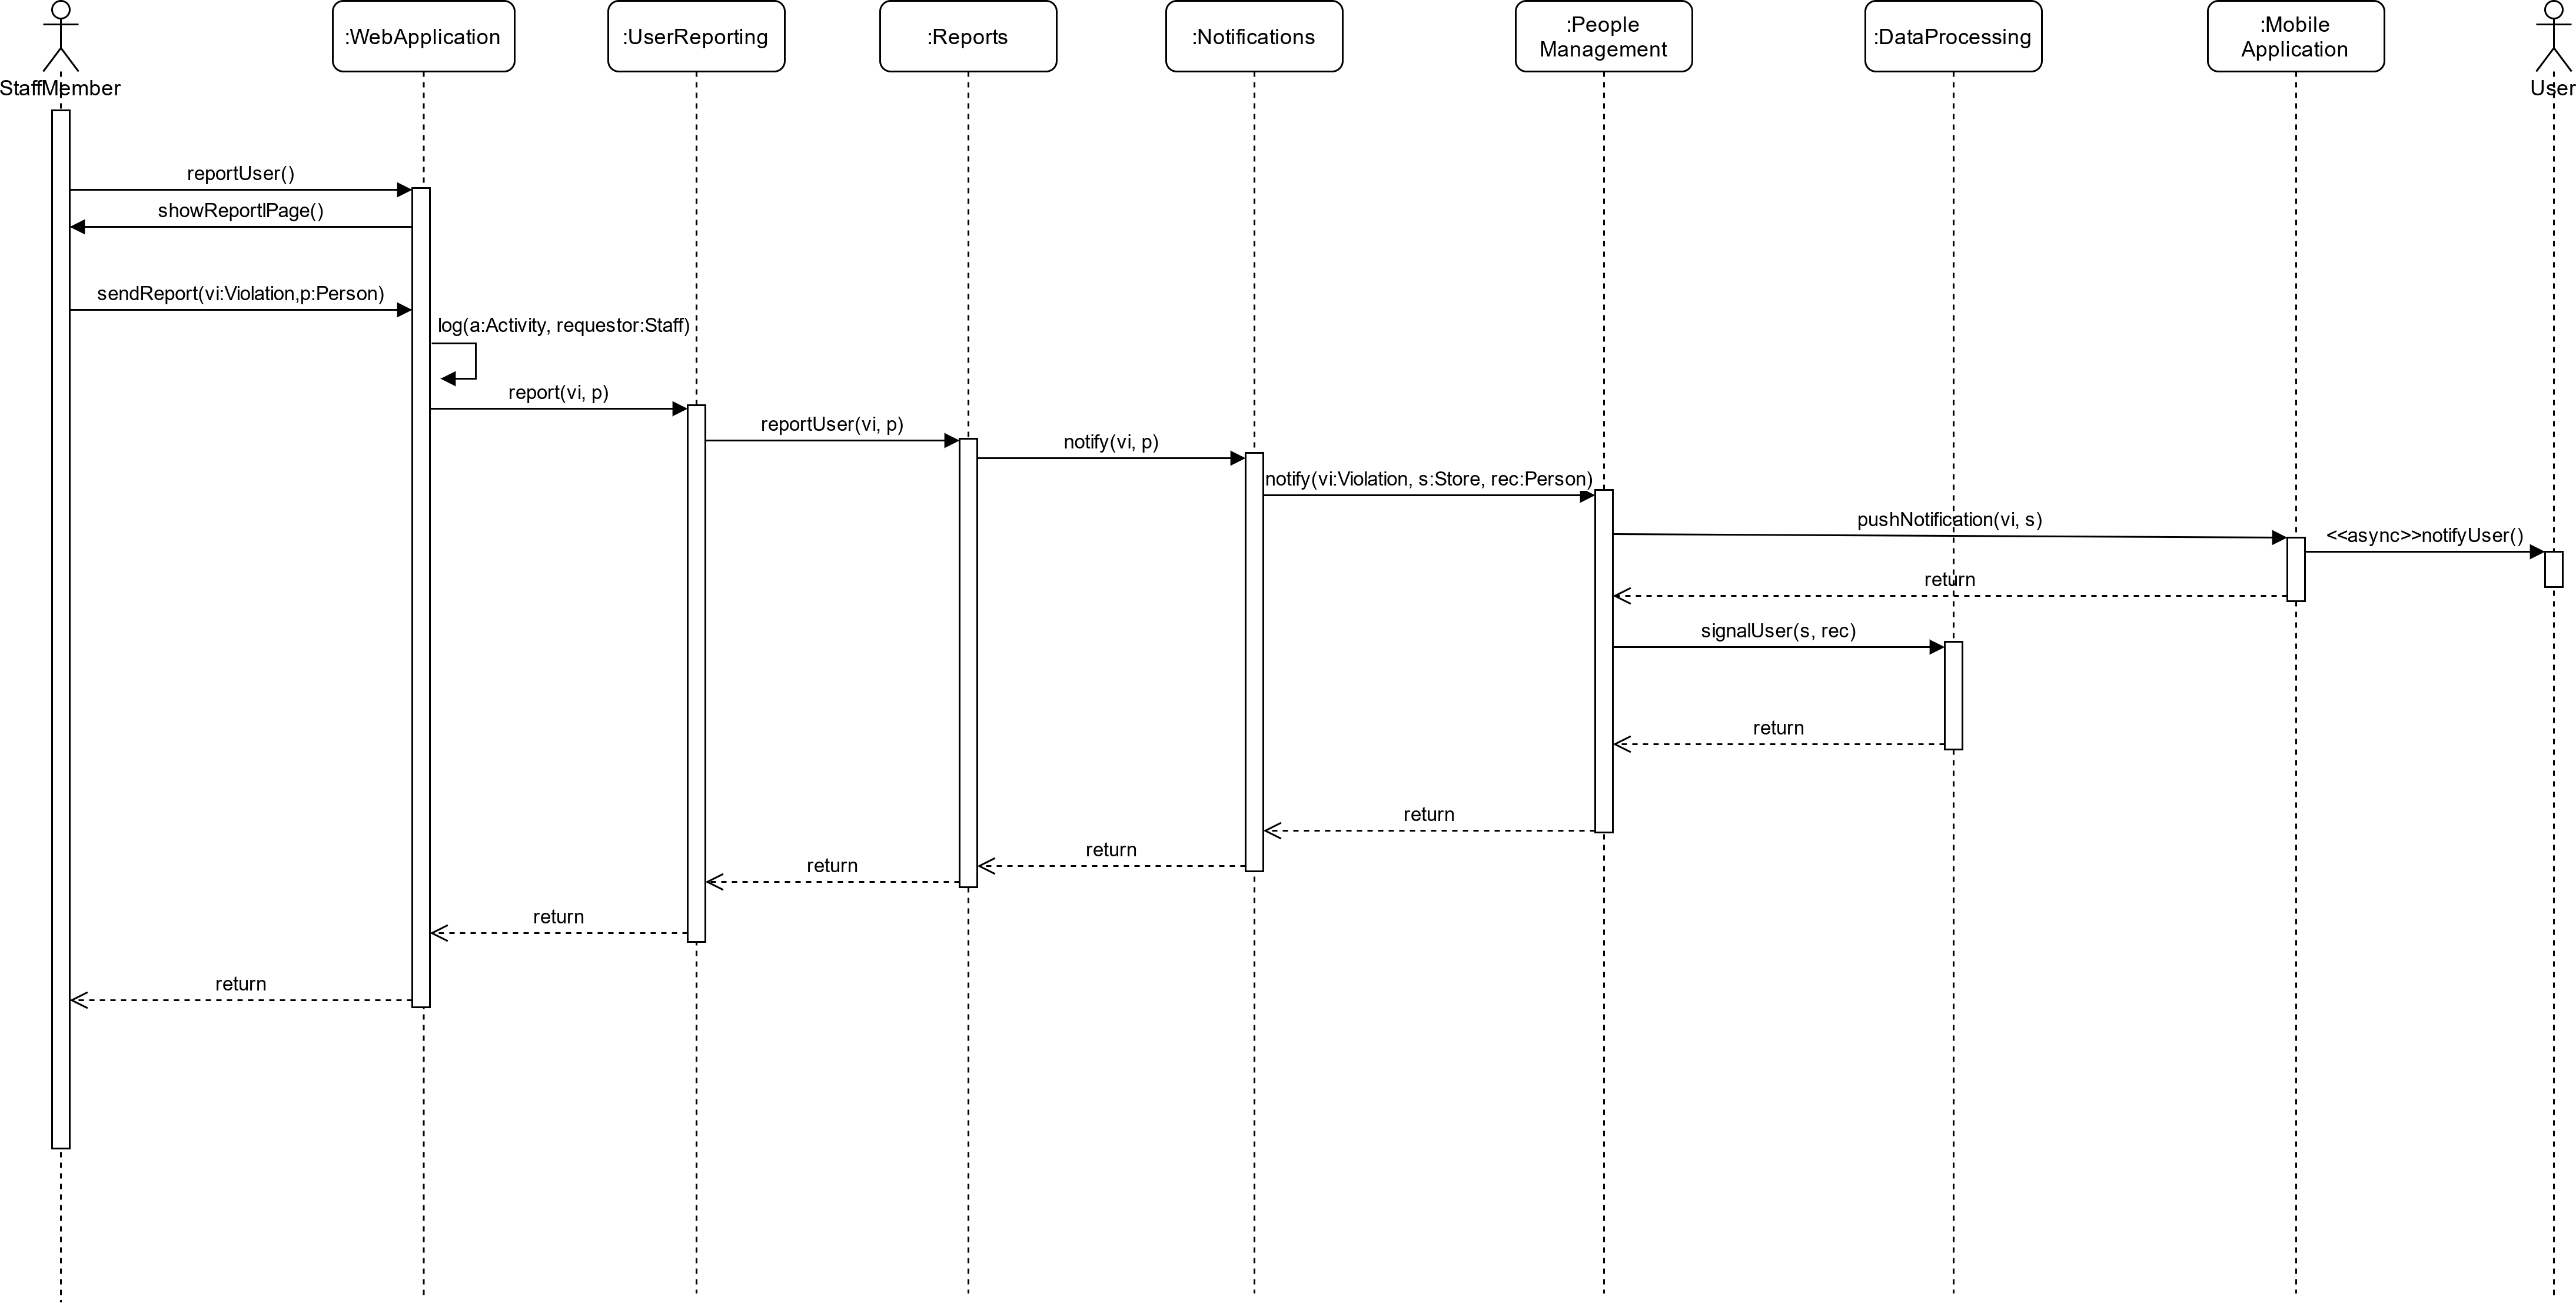
\includegraphics[width=\linewidth]{../Diagrams/Sequence/sequence_user_report.png}
	\caption{Sequence Diagram: User Report}
	\label{fig:sUserRep}
\end{figure}

\begin{figure}[H]
	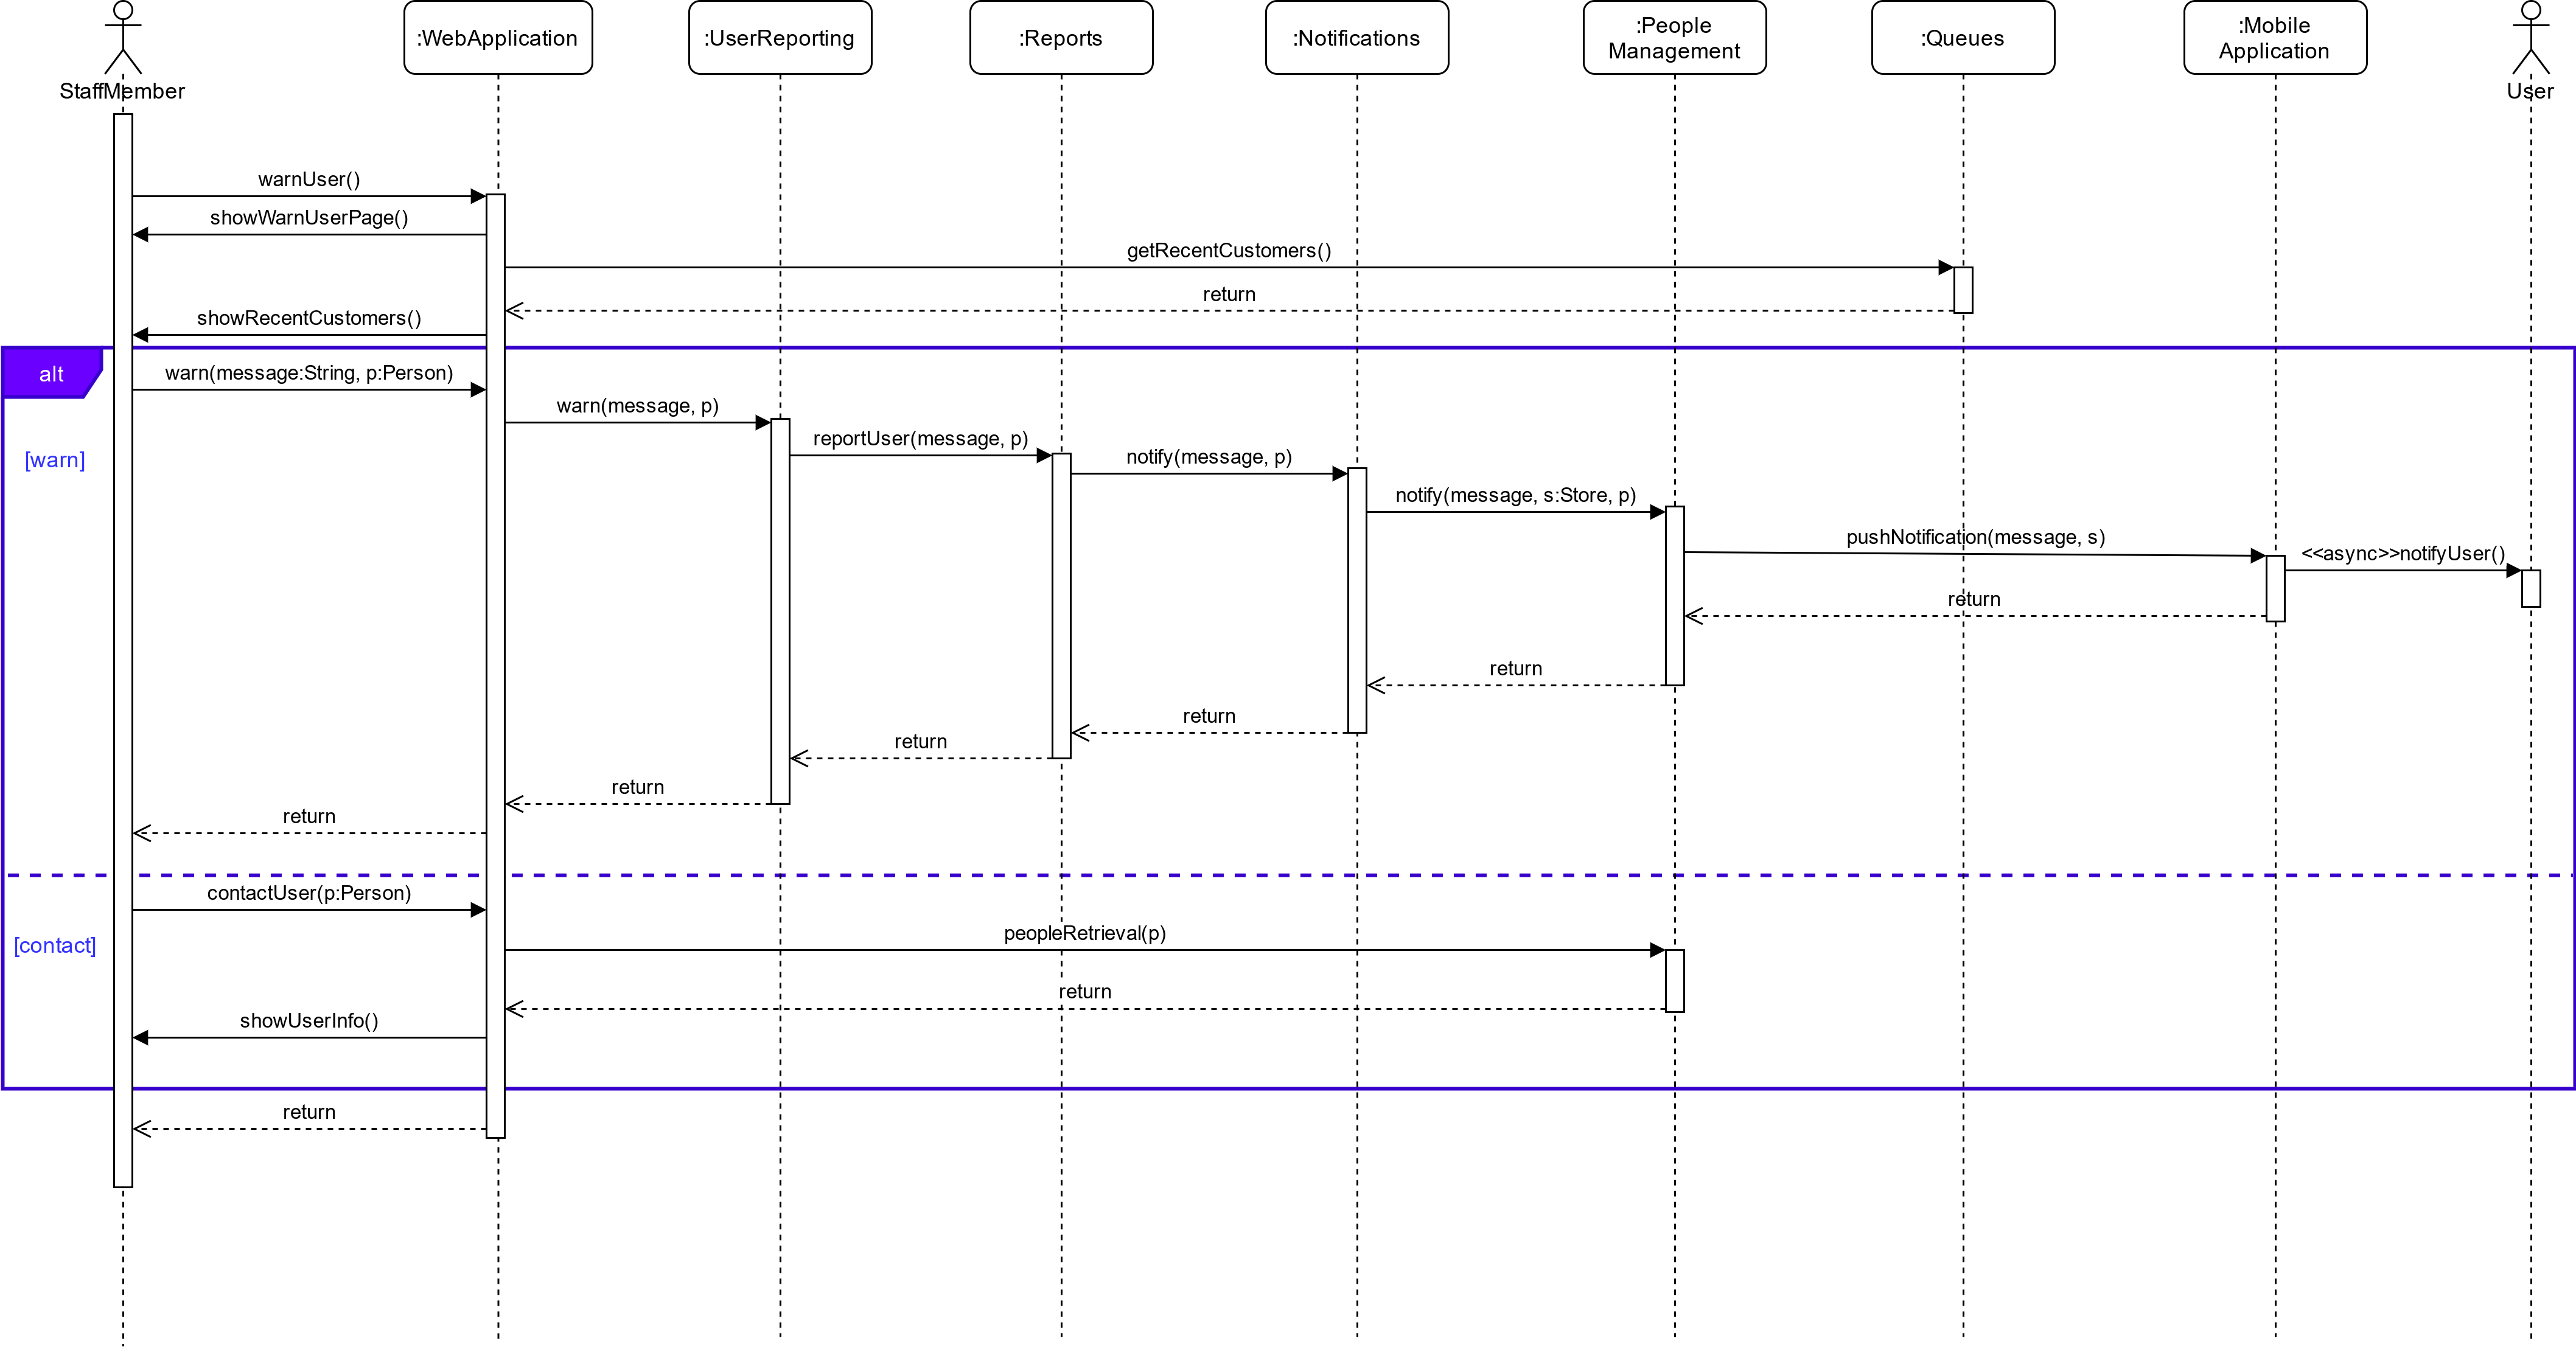
\includegraphics[width=\linewidth]{../Diagrams/Sequence/sequence_user_warn.png}
	\caption{Sequence Diagram: User Warn}
	\label{fig:sUserWarn}
\end{figure}

\subsection{Component interfaces}
\begin{figure}[H]
	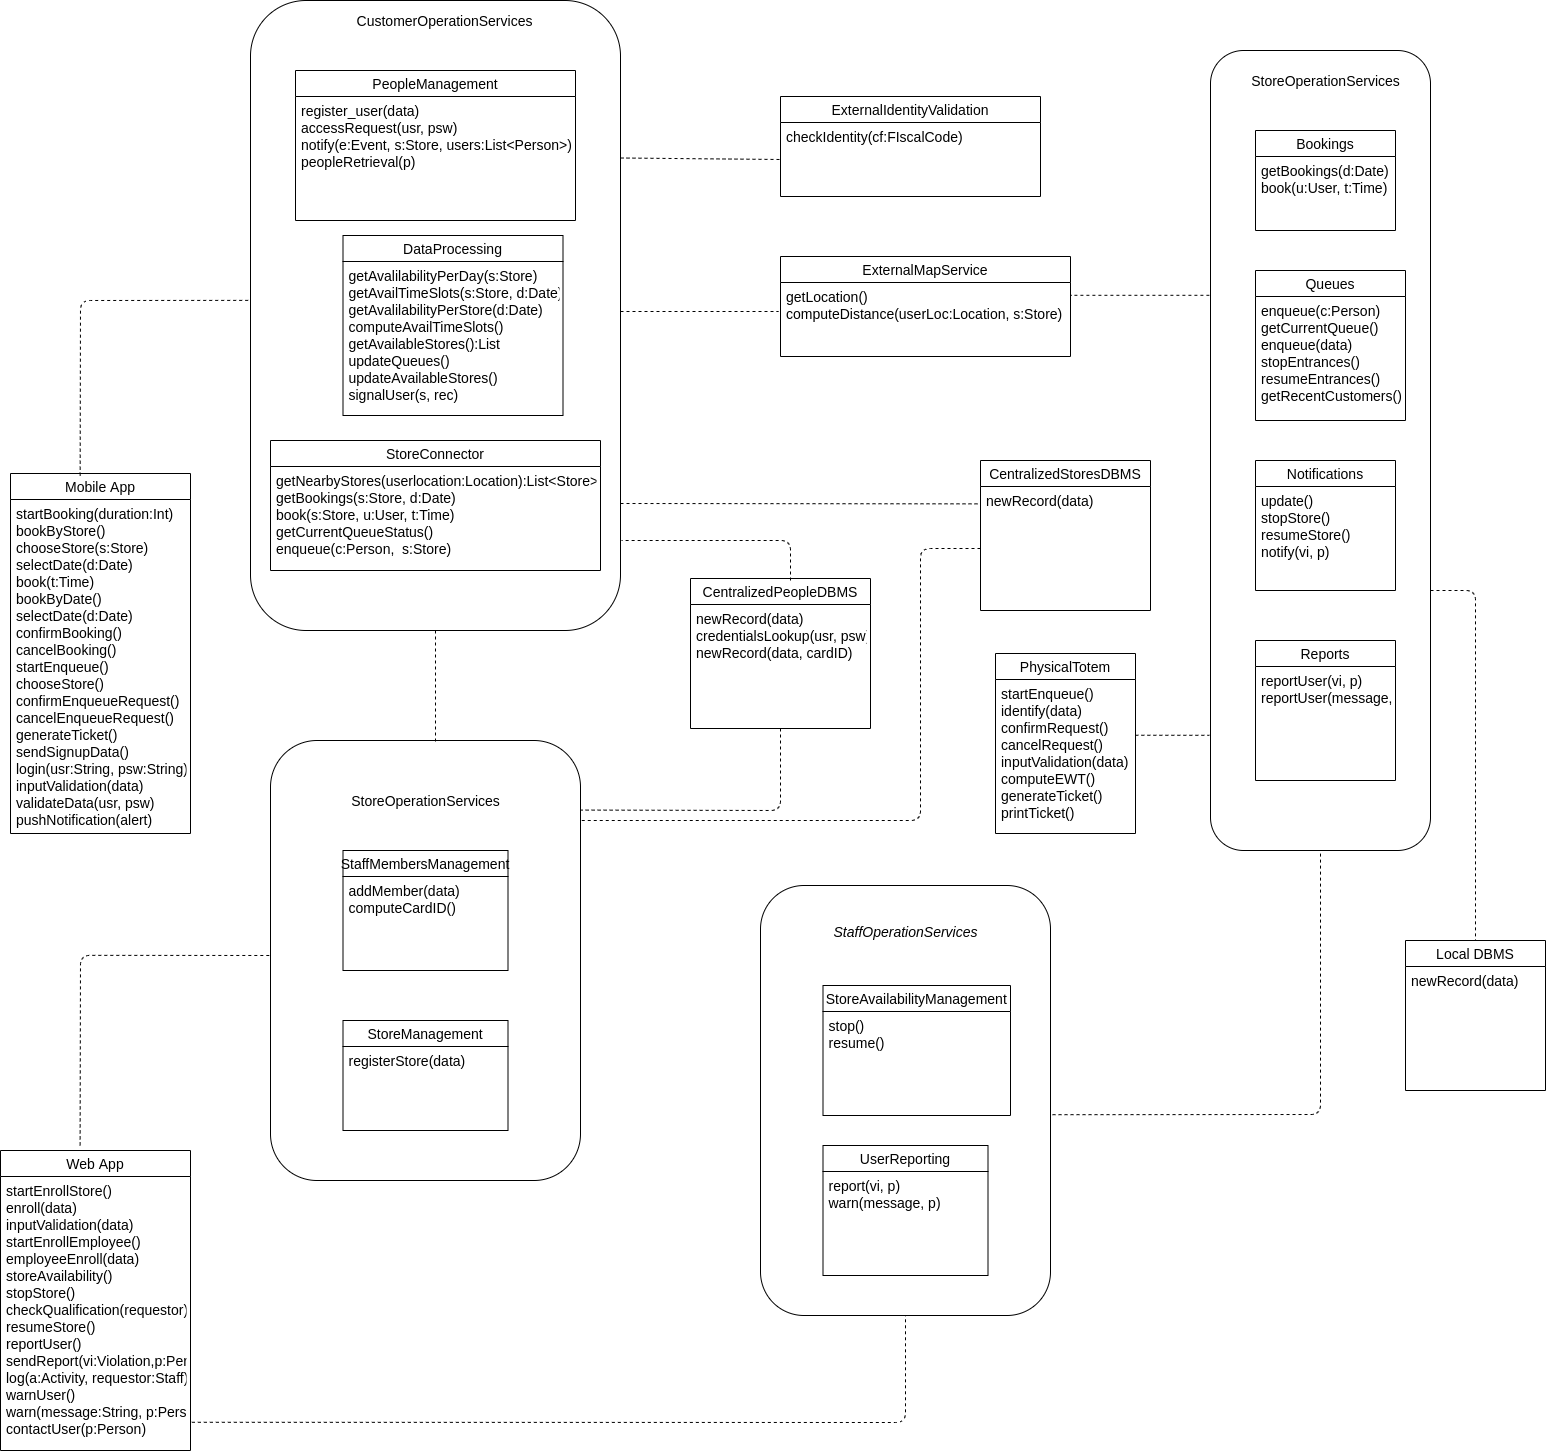
\includegraphics[width=\linewidth]{../Diagrams/Component Interface.png}
	\caption{Component Interface Diagram}
	\label{fig:CompInt}
\end{figure}
\subsection{Selected architectural styles and patterns}
\subsection{Other design decisions}
